% Options for packages loaded elsewhere
\PassOptionsToPackage{unicode}{hyperref}
\PassOptionsToPackage{hyphens}{url}
\PassOptionsToPackage{dvipsnames,svgnames,x11names}{xcolor}
%
\documentclass[
  12pt]{article}

\usepackage{amsmath,amssymb}
\usepackage{iftex}
\ifPDFTeX
  \usepackage[T1]{fontenc}
  \usepackage[utf8]{inputenc}
  \usepackage{textcomp} % provide euro and other symbols
\else % if luatex or xetex
  \usepackage{unicode-math}
  \defaultfontfeatures{Scale=MatchLowercase}
  \defaultfontfeatures[\rmfamily]{Ligatures=TeX,Scale=1}
\fi
\usepackage{lmodern}
\ifPDFTeX\else  
    % xetex/luatex font selection
\fi
% Use upquote if available, for straight quotes in verbatim environments
\IfFileExists{upquote.sty}{\usepackage{upquote}}{}
\IfFileExists{microtype.sty}{% use microtype if available
  \usepackage[]{microtype}
  \UseMicrotypeSet[protrusion]{basicmath} % disable protrusion for tt fonts
}{}
\makeatletter
\@ifundefined{KOMAClassName}{% if non-KOMA class
  \IfFileExists{parskip.sty}{%
    \usepackage{parskip}
  }{% else
    \setlength{\parindent}{0pt}
    \setlength{\parskip}{6pt plus 2pt minus 1pt}}
}{% if KOMA class
  \KOMAoptions{parskip=half}}
\makeatother
\usepackage{xcolor}
\setlength{\emergencystretch}{3em} % prevent overfull lines
\setcounter{secnumdepth}{5}
% Make \paragraph and \subparagraph free-standing
\makeatletter
\ifx\paragraph\undefined\else
  \let\oldparagraph\paragraph
  \renewcommand{\paragraph}{
    \@ifstar
      \xxxParagraphStar
      \xxxParagraphNoStar
  }
  \newcommand{\xxxParagraphStar}[1]{\oldparagraph*{#1}\mbox{}}
  \newcommand{\xxxParagraphNoStar}[1]{\oldparagraph{#1}\mbox{}}
\fi
\ifx\subparagraph\undefined\else
  \let\oldsubparagraph\subparagraph
  \renewcommand{\subparagraph}{
    \@ifstar
      \xxxSubParagraphStar
      \xxxSubParagraphNoStar
  }
  \newcommand{\xxxSubParagraphStar}[1]{\oldsubparagraph*{#1}\mbox{}}
  \newcommand{\xxxSubParagraphNoStar}[1]{\oldsubparagraph{#1}\mbox{}}
\fi
\makeatother


\providecommand{\tightlist}{%
  \setlength{\itemsep}{0pt}\setlength{\parskip}{0pt}}\usepackage{longtable,booktabs,array}
\usepackage{calc} % for calculating minipage widths
% Correct order of tables after \paragraph or \subparagraph
\usepackage{etoolbox}
\makeatletter
\patchcmd\longtable{\par}{\if@noskipsec\mbox{}\fi\par}{}{}
\makeatother
% Allow footnotes in longtable head/foot
\IfFileExists{footnotehyper.sty}{\usepackage{footnotehyper}}{\usepackage{footnote}}
\makesavenoteenv{longtable}
\usepackage{graphicx}
\makeatletter
\def\maxwidth{\ifdim\Gin@nat@width>\linewidth\linewidth\else\Gin@nat@width\fi}
\def\maxheight{\ifdim\Gin@nat@height>\textheight\textheight\else\Gin@nat@height\fi}
\makeatother
% Scale images if necessary, so that they will not overflow the page
% margins by default, and it is still possible to overwrite the defaults
% using explicit options in \includegraphics[width, height, ...]{}
\setkeys{Gin}{width=\maxwidth,height=\maxheight,keepaspectratio}
% Set default figure placement to htbp
\makeatletter
\def\fps@figure{htbp}
\makeatother

\addtolength{\oddsidemargin}{-.5in}%
\addtolength{\evensidemargin}{-1in}%
\addtolength{\textwidth}{1in}%
\addtolength{\textheight}{1.7in}%
\addtolength{\topmargin}{-1in}%
\usepackage{booktabs}
\usepackage{longtable}
\usepackage{array}
\usepackage{multirow}
\usepackage{wrapfig}
\usepackage{float}
\usepackage{colortbl}
\usepackage{pdflscape}
\usepackage{tabu}
\usepackage{threeparttable}
\usepackage{threeparttablex}
\usepackage[normalem]{ulem}
\usepackage{makecell}
\usepackage{xcolor}
\usepackage{amsmath}
\usepackage{float}
\usepackage{hyperref}
\usepackage[utf8]{inputenc}
\usepackage{bm}
\def\tightlist{}
\usepackage{setspace}
\newcommand\pD{$p\text{-}D$}
\newcommand\kD{$k\text{-}D$}
\newcommand\dD{$d\text{-}D$}
\newcommand\gD{$2\text{-}D$}
\makeatletter
\@ifpackageloaded{caption}{}{\usepackage{caption}}
\AtBeginDocument{%
\ifdefined\contentsname
  \renewcommand*\contentsname{Table of contents}
\else
  \newcommand\contentsname{Table of contents}
\fi
\ifdefined\listfigurename
  \renewcommand*\listfigurename{List of Figures}
\else
  \newcommand\listfigurename{List of Figures}
\fi
\ifdefined\listtablename
  \renewcommand*\listtablename{List of Tables}
\else
  \newcommand\listtablename{List of Tables}
\fi
\ifdefined\figurename
  \renewcommand*\figurename{Figure}
\else
  \newcommand\figurename{Figure}
\fi
\ifdefined\tablename
  \renewcommand*\tablename{Table}
\else
  \newcommand\tablename{Table}
\fi
}
\@ifpackageloaded{float}{}{\usepackage{float}}
\floatstyle{ruled}
\@ifundefined{c@chapter}{\newfloat{codelisting}{h}{lop}}{\newfloat{codelisting}{h}{lop}[chapter]}
\floatname{codelisting}{Listing}
\newcommand*\listoflistings{\listof{codelisting}{List of Listings}}
\makeatother
\makeatletter
\makeatother
\makeatletter
\@ifpackageloaded{caption}{}{\usepackage{caption}}
\@ifpackageloaded{subcaption}{}{\usepackage{subcaption}}
\makeatother

\ifLuaTeX
  \usepackage{selnolig}  % disable illegal ligatures
\fi
\usepackage[]{natbib}
\bibliographystyle{agsm}
\usepackage{bookmark}

\IfFileExists{xurl.sty}{\usepackage{xurl}}{} % add URL line breaks if available
\urlstyle{same} % disable monospaced font for URLs
\hypersetup{
  pdftitle={Looking at Non-Linear Dimension Reductions as Models in the Data Space},
  pdfauthor={Jayani P.G. Lakshika; Dianne Cook; Paul Harrison; Michael Lydeamore; Thiyanga S. Talagala},
  pdfkeywords={high-dimensional data, dimension reduction, hexagon
binning, low-dimensional representation, tour, data
vizualization, model-in-the-data-space},
  colorlinks=true,
  linkcolor={blue},
  filecolor={Maroon},
  citecolor={Blue},
  urlcolor={Blue},
  pdfcreator={LaTeX via pandoc}}



\begin{document}


\def\spacingset#1{\renewcommand{\baselinestretch}%
{#1}\small\normalsize} \spacingset{1}


%%%%%%%%%%%%%%%%%%%%%%%%%%%%%%%%%%%%%%%%%%%%%%%%%%%%%%%%%%%%%%%%%%%%%%%%%%%%%%

\title{\bf Looking at Non-Linear Dimension Reductions as Models in the
Data Space}
\author{
Jayani P.G. Lakshika\\
Econometrics \& Business Statistics, Monash University\\
and\\Dianne Cook\\
Econometrics \& Business Statistics, Monash University\\
and\\Paul Harrison\\
MGBP, BDInstitute, Monash University\\
and\\Michael Lydeamore\\
Econometrics \& Business Statistics, Monash University\\
and\\Thiyanga S. Talagala\\
Statistics, University of Sri Jayewardenepura\\
}
\maketitle

\bigskip
\bigskip
\begin{abstract}
Non-linear dimension reduction (NLDR) techniques such as tSNE, and UMAP
provide a low-dimensional representation of high-dimensional
(\(p\text{-}D\)) data using non-linear transformation. The methods and
parameter choices can create wildly different representations, making it
difficult to decide which is best, or whether any or all are accurate or
misleading. NLDR often exaggerates random patterns, sometimes due to the
samples observed. But NLDR views have an important role in data analysis
because, if done well, they provide a concise visual (and conceptual)
summary of \(p\text{-}D\) distributions. To help evaluate the NLDR we
have developed an algorithm to show the \(2\text{-}D\) NLDR model in the
\(p\text{-}D\) space, viewed with a tour. One can see if the model fits
everywhere or better in some subspaces, or completely mismatches the
data. It is used to evaluate which \(2\text{-}D\) layout is the best
representation of the \(p\text{-}D\) distribution and see how different
methods may have similar summaries or quirks.
\end{abstract}

\noindent%
{\it Keywords:} high-dimensional data, dimension reduction, hexagon
binning, low-dimensional representation, tour, data
vizualization, model-in-the-data-space
\vfill

\newpage
\spacingset{1.9} % DON'T change the spacing!


\spacingset{1.0}

\section{Introduction}\label{introduction}

Non-linear dimension reduction (NLDR) is popular for making a convenient
low-dimensional (\kD{}) representation of high-dimensional (\pD{}) data.
Recently developed methods include t-distributed stochastic neighbor
embedding (tSNE) \citep{laurens2008}, uniform manifold approximation and
projection (UMAP) \citep{leland2018}, potential of heat-diffusion for
affinity-based trajectory embedding (PHATE) algorithm \citep{moon2019},
large-scale dimensionality reduction Using triplets (TriMAP)
\citep{amid2022}, and pairwise controlled manifold approximation
(PaCMAP) \citep{yingfan2021}. However, the representation generated can
vary dramatically from method to method, and with different choices of
parameters or random seeds made using the same method
(Figure~\ref{fig-NLDR-variety}). The dilemma for the analyst is then,
\textbf{which representation to use}. The choice might result in
different procedures used in the downstream analysis, or different
inferential conclusions. The research described here provides new visual
tools to aid with this decision.

\begin{figure}

\centering{

\includegraphics[width=1\textwidth,height=\textheight]{paper_files/figure-pdf/fig-NLDR-variety-1.pdf}

}

\caption{\label{fig-NLDR-variety}Six different NLDR representations of
the same data. Different techniques and different parameter choices are
used. Researchers may have seen any of these in their analysis of this
data, depending on their choice of method, or typical parameter choice.
Would they make different decisions downstream in the analysis depending
on which version seen? Which is the most accurate representation of the
structure in high dimensions?}

\end{figure}%

The paper is organised as follows. Section~\ref{sec-background} provides
a summary of the literature on NLDR, and high-dimensional data
visualization methods. Section~\ref{sec-method} contains the details of
the new methodology, including simulated data examples. Two applications
illustrating the use of the new methodology for bioinformatics and image
classification are in Section~\ref{sec-applications}. Limitations and
future directions are provided in Section~\ref{sec-discussion}.

\section{Background}\label{sec-background}

Historically, \kD{} representations of \pD{} data have been computed
using multidimensional scaling (MDS) \citep{borg2005}, which includes
principal components analysis (PCA) \citep{jolliffe2011} as a special
case. The \kD{} representation can be considered to be a layout of
points in \kD{} produced by an embedding procedure that maps the data
from \pD{}. In MDS, the \kD{} layout is constructed by minimizing a
stress function that differences distances between points in \pD{} with
potential distances between points in \kD{}. Various formulations of the
stress function result in non-metric scaling \citep{saeed2018} and
isomap \citep{silva2002}. Challenges in working with high-dimensional
data, including visualization, are outlined in \citet{johnstone2009}.

Many new methods for NLDR have emerged in recent years, all designed to
better capture specific structures potentially existing in \pD{}. Here
we focus on five currently popular techniques, tSNE, UMAP, PHATE, TriMAP
and PaCMAP. tNSE and UMAP can be considered to produce the \kD{}
minimizing the divergence between two distributions, where the
distributions are modeling the inter-point distances. PHATE, TriMAP and
PaCMAP are examples of diffusion processes \citep{coifman2005} spreading
to capture geometric shapes, that include both global and local
structure.

The array of layouts in Figure~\ref{fig-NLDR-variety} illustrate what
can emerge from the choices of method and parameters, and the random
seed that initiates the computation. Key structures interpreted from
these views suggest: (1) highly \textbf{separated clusters} (a, b, e, g,
h) with the number ranging from 3-6; (2) \textbf{stringy branches} (f),
and (3) \textbf{barely separated clusters} (c, d) which would
\textbf{contradict} the other representations.

It happens because these methods and parameter choices provide different
lenses on the interpoint distances in the data.

The alternative approach to visualizing the high-dimensional data is to
use linear projections. PCA is the classical approach, resulting in a
set of new variables which are linear combinations of the original
variables. Tours, defined by \citet{lee2021}, broaden the scope by
providing movies of linear projections, that provide views the data from
all directions. \citet{lee2021} provides an review of the main
developments in tours. There are many tour algorithms implemented, with
many available in the R package \texttt{tourr} \citep{wickham2011}, and
versions enabling better interactivity in \texttt{langevitour}
\citep{harisson2024} and \texttt{detourr} \citep{hart2022}. Linear
projections are a safe way to view high-dimensional data, because they
do not warp the space, so they are more faithful representations of the
structure. However, linear projections can be cluttered, and global
patterns can obscure local structure. The simple activity of projecting
data from \pD{} suffers from piling \citep{laa2022}, where data
concentrates in the center of projections. NLDR is designed to escape
these issues, to exaggerate structure so that it can be observed. But as
a result NLDR can hallucinate wildly, to suggest patterns that are not
actually present in the data.

The solution is to use the tour to examine how the NLDR is warping the
space. This approach follows what \citet{wickham2015} describes as
\emph{model-in-the-data-space}. The fitted model should be overlaid on
the data, to examine the fit relative the spread of the observations.
While this is straightforward, and commonly done when data is \gD{}, it
is also possible in \pD{}, for many models, when a tour is used.

\citet{wickham2015} provides several examples of models overlaid on the
data in \pD{}. In hierarchical clustering, a representation of the
dendrogrom using points and lines can be constructed by augmenting the
data with points marking merging of clusters. Showing the movie of
linear projections reveals shows how the algorithm sequentially fitted
the cluster model to the data. For linear discriminant analysis or
model-based clustering the model can be indicated by \((p-1)\text{-}D\)
ellipses. It is possible to see whether the elliptical shapes
appropriately matches the variance of the relevant clusters, and to
compare and contrast different fits. For PCA, one can display the \kD{}
plane of the reduced dimension using wireframes of transformed cubes.
Using a wireframe is the approach we take here, to represent the NLDR
model in \pD{}.

\section{Method}\label{sec-method}

\subsection{What is the NLDR model?}\label{what-is-the-nldr-model}

At first glance, thinking of NLDR as a modeling technique might seem
strange. It is a simplified representation or abstraction of a system,
process, or phenomenon in the real world. The \pD{} observations are the
realization of the phenomenon, and the \kD{} NLDR layout is the
simplified representation. From a statistical perspective we can
consider the distances between points in the \kD{} layout to be variance
that the model explains, and the (relative) difference with their
distances in \pD{} is the error, or unexplained variance. We can also
imagine that the positioning of points in \gD{} represent the fitted
values, that will have some prescribed position in \pD{} that can be
compared with their observed values. This is the conceptual framework
underlying the more formal versions of factor analysis \citep{cfa69} and
multidimensional scaling (MDS) \citep{borg2005}. (Note that, for this
thinking the full \pD{} data needs to be available, not just the
interpoint distances.)

\begin{table}

\centering{

\centering\begingroup\fontsize{12}{14}\selectfont

\begin{tabular}{>{\raggedright\arraybackslash}p{3cm}>{\raggedright\arraybackslash}p{12cm}}
\toprule
\textbf{Notation} & \textbf{Description}\\
\midrule
$n, p, k$ & number of observations, variables, embedding dimension, respectively\\
$\mathbfit{X}, \mathbfit{x}$ & $p$-dimensional data (population, sample)\\
$\mathbfit{y}$ & $k$-dimensional layout\\
$P$ & orthonormal basis, generating a $d\text{-}dimensional$ linear projection of $p$-dimensional data\\
$T$ & true  model\\
\addlinespace
$g$ & functional mapping from \pD{} to \kD{}, especially as prescribed by NLDR\\
$\mathbfit{\theta}$ & (Hyper-) parameters for NLDR method\\
$r$ & ranges of the embedding components\\
$C^{(j)}$ & $j$-dimensional bin centers\\
$(b_1, b_2)$ & number of bins in each direction\\
\addlinespace
$(a_1, a_2)$ & binwidths, distance between centroids in each direction\\
$(s_1, \ s_2)$ & starting coordinates of the hexagonal grid\\
$q$ & buffer to ensure hexgrid covers data, proportion of data range, 0-1\\
$m$ & number of non-empty bins\\
$b$ & number of  hexagons in the grid\\
\addlinespace
$h$ & hexagonal id\\
\bottomrule
\end{tabular}
\endgroup{}

}

\caption{\label{tbl-notation}Summary of notation for describing new
methodology.}

\end{table}%

We define the NLDR as a function
\(g\text{:}~ \mathbb{R}^{n\times p} \rightarrow \mathbb{R}^{n\times k}\),
with (hyper-)parameters \(\mathbfit{\theta}\). The parameters,
\(\mathbfit{\theta}\), depend on the choice of \(g\), and can be
considered part of model fitting in the traditional sense. Common
choices for \(g\) include functions used in tSNE, UMAP, PHATE, TriMAP,
PaCMAP, or MDS, although in theory any function that does this mapping
is suitable.

With our goal being to make a representation of this \gD{} layout that
can be lifted into high-dimensional space, the layout needs to be
augmented to include neighbour information. A simple approach would be
to triangulate the points and add edges. A more stable approach is to
first hexagonly bin the data, reducing it from \(n\) to \(m\leq n\)
observations, and connect the bin centroids. This process serves to
reduce some noisiness in the resulting surface shown in \pD{}. The steps
in this process are shown in Figure~\ref{fig-NLDR-scurve}, and
documented below.

To illustrate the method, we use \(7\text{-}D\) simulated data, which we
call the ``S-curve''. It is constructed by simulating \(n=750\)
observations from \(\theta \sim U(-3\pi/2, 3\pi/2)\),
\(X_1 = \sin(\theta)\), \(X_2 \sim U(0, 2)\) (adding thickness to the
S), \(X_3 = \text{sign}(\theta) \times (\cos(\theta) - 1)\). The
remaining variables \(X_4, X_5, X_6, X_7\) are all uniform error, with
small variance. We would consider \(T=(X_1, X_2, X_3)\) to be the
geometric structure (true model) that we hope to capture.

\begin{figure}[H]

\begin{minipage}{0.33\linewidth}
\begin{center}
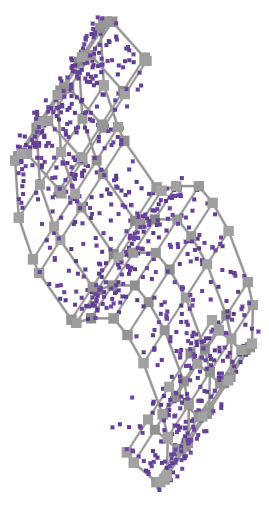
\includegraphics[width=1.5625in,height=\textheight]{figures/scurve/sc_true_1.png}
\end{center}
\end{minipage}%
%
\begin{minipage}{0.33\linewidth}
\begin{center}
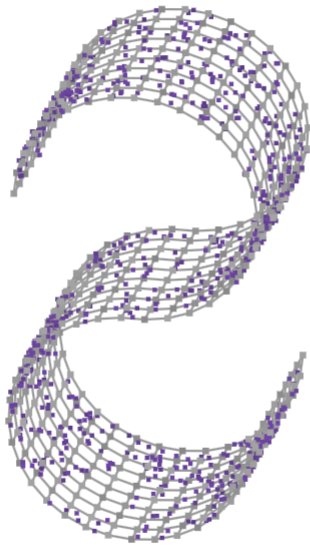
\includegraphics[width=1.5625in,height=\textheight]{figures/scurve/sc_true_2.png}
\end{center}
\end{minipage}%
%
\begin{minipage}{0.33\linewidth}
\begin{center}
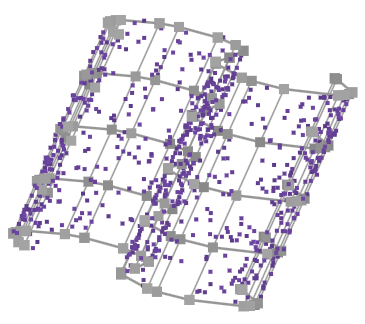
\includegraphics[width=1.5625in,height=\textheight]{figures/scurve/sc_true_3.png}
\end{center}
\end{minipage}%

\caption{\label{fig-scurve-true-sc}Three views of the true model in
projections from \(7\text{-}D\), for the S-curve data. The model closely
fits the shape. (The \textbf{langevitour} software is used to view the
data with a tour, and the full video is available at
\url{https://youtu.be/I5GL23vLiw0}).}

\end{figure}%

\begin{figure}

\centering{

\includegraphics[width=1\textwidth,height=\textheight]{paper_files/figure-pdf/fig-NLDR-scurve-1.pdf}

}

\caption{\label{fig-NLDR-scurve}Key steps for constructing the model on
the UMAP layout (\(k=2\)): (a) data, (b) hexagon bins, (c) bin
centroids, and (d) triangulated centroids. The S-curve data is shown.}

\end{figure}%

\subsection{Algorithm to represent the model in
2D}\label{algorithm-to-represent-the-model-in-2d}

\subsubsection{Scale the data}\label{scale-the-data}

Because we are working with distances between points, starting with data
having a standard scale, e.g.~{[}0, 1{]}, is recommended. The default
should take the aspect ratio produced by the NLDR
\((r_1, r_2, ..., r_k)\) into account. When \(k=2\), as in hexagon
binning, the default range is \([0, y_{i,\text{max}}], i=1,2\), where
\(y_{1,\text{max}}=1\) and \(y_{2,\text{max}} = \frac{r_2}{r_1}\)
(Figure~\ref{fig-NLDR-scurve}). If the NLDR aspect ratio is ignored then
set \(y_ {2,\text{max}} = 1\).

\subsubsection{Computing hexagon grid
configuration}\label{computing-hexagon-grid-configuration}

Although there are several implementations of hexagon binning
\citep{carr1987}, and a published paper \citep{dan2023}, surprisingly,
none has sufficient detail or components that produce everything needed
for this project. So we described the process used here.
Figure~\ref{fig-hex-param} illustrates the notation used.

The \gD{} hexagon grid is defined by its bin centroids. Each hexagon,
\(H_h\) (\(h = 1, \dots, b\)) is uniquely described by centroid,
\(C_{h}^{(2)} = (c_{h1}, c_{h2})\). The number of bins in each direction
is denoted as \((b_1, b_2)\), with \(b = b_1 \times b_2\) being the
total number of bins. We expect the user to provide just \(b_1\) and we
calculate \(b_2\) using the NLDR ratio, to compute the grid.

To ensure that the grid covers the range of data values a buffer
parameter (\(q\)) is set as a proportion of the range. By default,
\(q=0.1\). The buffer should be extending a full hexagon width (\(a_1\))
and height (\(a_2\)) beyond the data, in all directions. The lower left
position where the grid starts is defined as \((s_1, s_2)\), and
corresponds to the centroid of the lowest left hexagon,
\(C_{1}^{(2)} = (c_{11}, c_{12})\). This must be smaller than the
minimum data value. Because it is one buffer unit, \(q\) below the
minimum data values, \(s_1 = -q\) and \(s_2 = -qr_2\).

The value for \(b_2\) is computed by fixing \(b_1\). Considering the
upper bound of the first NLDR component, \(a_1 > \frac{1+2q}{b_1 -1}\).
Similarly, for the second NLDR component,
\(a_2 > \frac{r_2 + q(1 + r_2)}{(b_2 - 1)}\). Since
\(a_2 = \frac{\sqrt(3)}{2}a_1\) for regular hexagons,
\(a_1 > \frac{2[r_2 + q(1 + r_2)]}{\sqrt{3}(b_2 - 1)}\). This is a
linear optimization problem. Therefore, the optimal solution must occur
on a vertex. Therefore,
\(b_2 = \Big\lceil1 +\frac{2[r_2 + q(1 + r_2)](b_1 - 1)}{\sqrt{3}(1 + 2q)}\Big\rceil\).

\begin{figure}[H]

\centering{

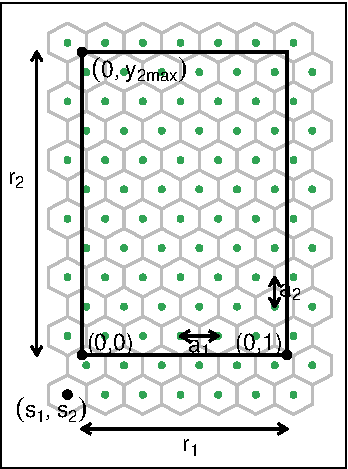
\includegraphics[width=1\textwidth,height=0.3\textheight]{paper_files/figure-pdf/fig-hex-param-1.pdf}

}

\caption{\label{fig-hex-param}The components of the hexagon grid
illustrating notation.}

\end{figure}%

\subsubsection{Binning the data}\label{binning-the-data}

Observations are grouped into bins based on their nearest centroid. This
produces a reduction in size of the data from \(n\) to \(m\), where
\(m\leq b\) (total number of bins). This can be defined using the
function
\(u: \mathbb{R}^{n\times 2} \rightarrow \mathbb{R}^{m\times 2}\), where
\(u(i) = \arg\min_{j = 1, \dots, b} \sqrt{(y_{i1} - C^{(2)}_{j1})^2 + (y_{i2} - C^{(2)}_{j2})^2}\),
mapping observation \(i\) into \(H_h = \{i| u(i) = h\}\).

By default, the bin centroid is used for describing a hexagon (as done
in Figure~\ref{fig-NLDR-scurve} (c)), but any measure of center, such as
a mean or weighted mean of the points within each hexagon, could be
used. The bin centers, and the binned data, are the two important
components needed to render the model representation in high dimensions.

\subsubsection{Indicating neighborhood}\label{indicating-neighborhood}

Delaunay triangulation \citep{lee1980, alb2024} is used to connect
neighboring centroids. The edges are needed to preserve neighborhood
information when the model is lifted into \pD{}.

When shapes are non-linear in the NLDR layout, some edges could be long.
It is unlikely

It can also happen that distant centroids can be connected, which can
result in long line segments. In order to generate a smooth surface in
\gD{}, these long line segments must be removed
(Figure~\ref{fig-NLDR-scurve} (d)).

\subsection{\texorpdfstring{Rendering the model in
\pD{}}{Rendering the model in }}\label{rendering-the-model-in}

The last step is to lift the \kD{} model into \pD{} by computing \pD{}
vectors that represent bin centroids. We use the \pD{} mean of the
points in \(H_h\) to map the centroid \(C_{h}^{(2)} = (c_{h1}, c_{h2})\)
to a point in \pD{}. Let the \pD{} mean be

\[C_{h}^{(p)} = \frac{1}{n_h}\sum_{i =1}^{n_h} x_i, h = {1, \dots, b; n_h > 0}.\]
Furthermore, line segments that exist in the \kD{} model generate line
segments in \pD{} by connecting the \pD{} means of the corresponding
\kD{} bin centroids.

XXXAdd best fit with UMAP and discuss why it's the best fit

XXX Should there be a second long edge removal? You can compute the
edges in \pD{} now, and if there are long edges maybe these should be
pruned, and we re-plot the \gD{} view.

\subsection{Measuring the fit}\label{sec-summary}

The model here is similar to a confirmatory factor analysis model
\citep{brown2015}, \(\widehat{T}(X_1, X_2, X_3) + \Epsilon\). The
difference between the fitted model and observed values would be
considered to be residuals, and for this problem are \(7\text{-}D\).

Observations are associated with their bin center, \(C_{h}^{(p)}\),
which are also considered to be the \emph{fitted values}. These can also
be denoted as \(\widehat{X}\).

The error is computed by taking the squared \pD{} Euclidean distance,
corresponding to computing the mean squared error (MSE) as:

\begin{equation}\phantomsection\label{eq-equation1}{\frac{1}{n}\sum_{h = 1}^{b}\sum_{i = 1}^{n_h}\sum_{j = 1}^{p} (\mathbfit{x}_{hij} - C^{(p)}_{hj})^2}\end{equation}

where \(n\) is the number of observations, \(b\) is the number of bins,
\(n_h\) is the number of observations in \(h^{th}\) bin, \(p\) is the
number of variables, \(\mathbfit{x}_{hij}\) is the \(j^{th}\)
dimensional data of \(i^{th}\) observation in \(h^{th}\) hexagon.

\subsection{\texorpdfstring{Prediction into
\gD{}}{Prediction into }}\label{prediction-into}

A new benefit of this fitted model is that it allows us to now predict a
new observation's value in the NLDR, for any method. The steps are to
determine the closest bin center in \pD{}, \(C^{(p)}_{h}\) and predict
it to be the centroid of this bin in \gD{}, \(C^{(2)}_{h}\). This can be
written as, let
\(z(i) = \arg\min_{j = 1, \dots, b} \sqrt{\sum_{v=1}^{p}(x_{iv} - C^{(p)}_{jv})^2}\),
then the new observation \(i\) falls in the hexagon,
\(H_h = \{i| z(i) = h\}\) and the corresponding \kD{} bin centroids,
\(C_{h}^{(2)} = (c_{h1}, c_{h2})\).

\begin{figure}[H]

\begin{minipage}{0.50\linewidth}
\begin{center}
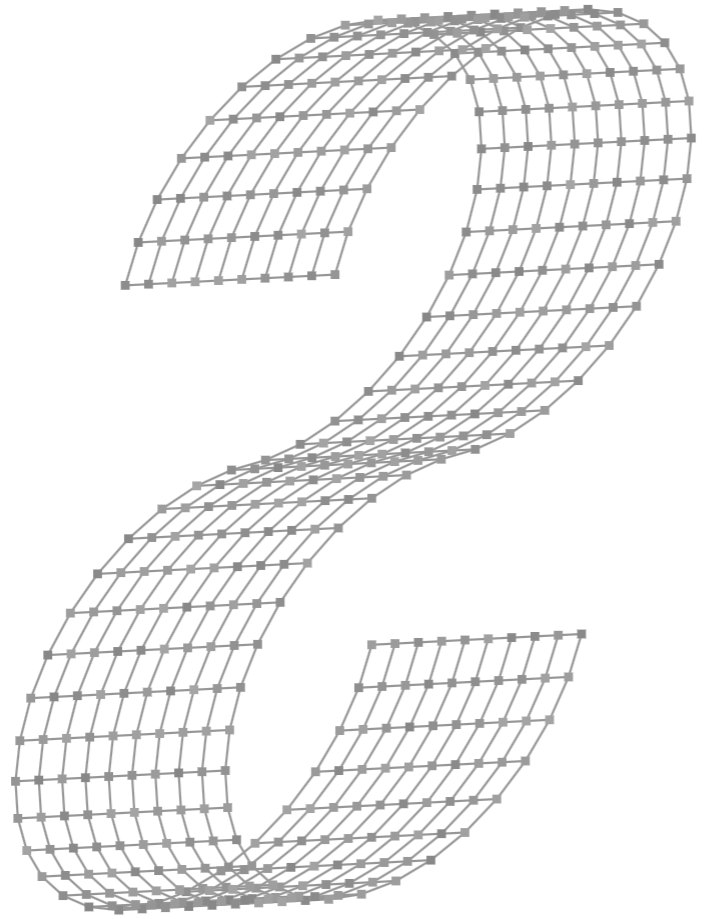
\includegraphics[width=1.5625in,height=\textheight]{figures/scurve/sc_true_only.png}
\end{center}
\end{minipage}%
%
\begin{minipage}{0.50\linewidth}
\begin{center}
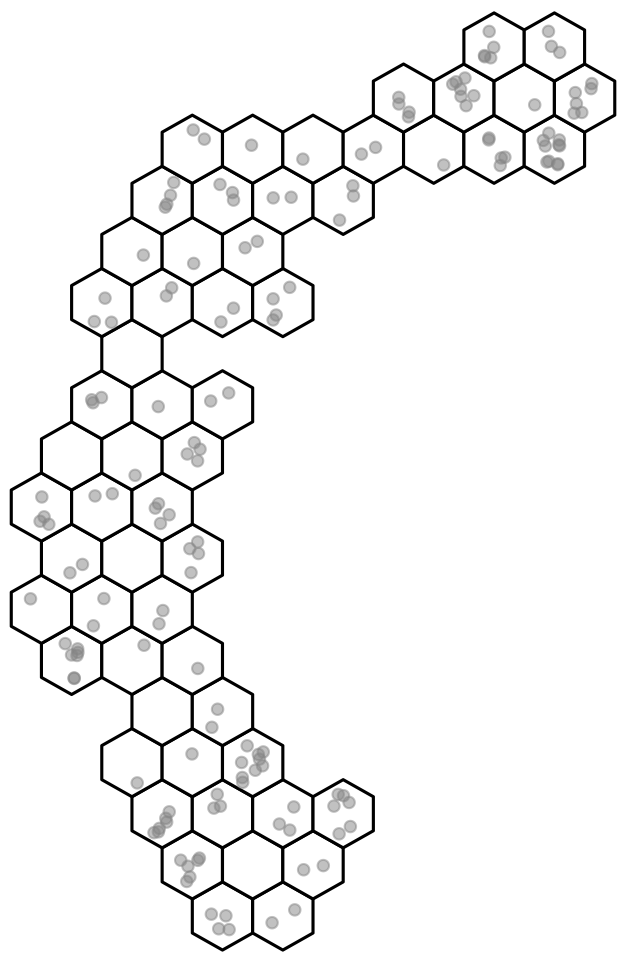
\includegraphics[width=1.5625in,height=\textheight]{figures/scurve/pred_true_view.png}
\end{center}
\end{minipage}%

\caption{\label{fig-scurve-pred-sc}A view of the true model in
projections from \(7\text{-}D\), and predictions of the true model in
\gD{}, for the S-curve data. The predictions fits the UMAP layout which
means that it capture the geometry of S-curve with UMAP.}

\end{figure}%

XXX Prediction should have a jitter option, to spread the predicted
points out fully in the hexagons.

\subsection{Tuning}\label{tuning}

The performance and robustness of our model depend on four key
parameters: (i) bin start position \((s_1, \ s_2)\), (ii) the total
number of bins (\(b\)), (iii) a benchmark value used to remove
low-density hexagons, and (iv) a benchmark value used to remove long
edges. However, there is no analytical formula to calculate appropriate
values for these parameters. The selection of these parameter values
depends on the model performance computed by MSE
(Section~\ref{sec-summary}), except for the threshold used to remove
long edges.

\subsubsection{Bin start position and number of
bins}\label{bin-start-position-and-number-of-bins}

The starting position of the hexagonal grid is important because
different starting points result in different distributions of data
across bins, even with the same total number of bins. This variation
affects the model due to the differing number of non-empty bins.
Therefore, it is necessary to evaluate various starting points with
different total numbers of bins to determine which configurations are
more effective at capturing the structure and fitting the model.

\begin{figure}[H]

\centering{

\includegraphics[width=1\textwidth,height=\textheight]{paper_files/figure-pdf/fig-bins-scurve-1.pdf}

}

\caption{\label{fig-bins-scurve}Hexbin density plots of UMAP layout of
the S-curve data, using three different bin inputs: (a)
\(b = 91 \text{ } (7, \text{ }13)  \text{ }(q = 0.12)\), (b)
\(b = 220 \text{ } (11, \text{ }20) \text{ }(q = 0.07)\), and (c)
\(b = 527 \text{ } (17, \text{ }31) \text{ }(q = 0.05)\). Color
indicates standardized counts, dark indicating high count and light
indicates low count. At the smallest bin size the data segregates into
two separate groups, suggesting this is too many bins. Using the MSE of
the model fit in \(p\text{-}D\) helps decide on a useful choice of
number of bins.}

\end{figure}%

To determine the effective \(b\), candidate values are selected based on
the range between the minimum and approximate maximum \(b_1\), because
\(b_2\) is computed from \(b_1\). The minimum \(b_1\) is set to \(2\),
while the maximum number is estimated by taking the square root of
\(\frac{n}{2}\). By evaluating MSE across varying \(b\) within this
range for different \(q\), helps to determine an appropriate values for
\(b\) and \(q\) (Figure~\ref{fig-param-scurve} (a)).

\subsubsection{Removal of low density
bins}\label{removal-of-low-density-bins}

Once setting up the hexagon grid with an appropriate number of bins,
some hexagon bins may have few or no data points within them
(Figure~\ref{fig-bins-scurve} (b)). To ensure comprehensive coverage of
the NLDR data, it is necessary to select hexagon bins with a
considerable number of data points. This involves calculating the number
of points within each hexagon. Then, the standard count is computed by
dividing the number of points within each hexagon by the maximum number
of points in the grid. Next, bins with a standard count less than a
benchmark value are removed (Figure~\ref{fig-param-scurve} (c)). There
is no specific rule for selecting a benchmark value. However, the
following steps can help determine a suitable value for removing
low-density hexagons:

\begin{enumerate}
\def\labelenumi{\arabic{enumi}.}
\tightlist
\item
  Plot the distribution of the standardized counts
  (Figure~\ref{fig-param-scurve} (b)).
\item
  Examine the distribution of counts.
\item
  Select the first quantile value if the distribution is skewed.
\end{enumerate}

The benchmark value for removing low-density hexagons ranges between
\(0\) and \(1\). When analyzing how these benchmark values influence
model performance, it's essential to observe the change in MSE as the
benchmark value increases (see \textbf{?@fig-mse-scurve-lwd}). The MSE
shows a gradual increase as the benchmark value progresses from \(0\) to
\(1\). Evaluating this rate of increase is important. If the increment
is not considerable, the decision might lean towards retaining
low-density hexagons.

Furthermore, selecting the benchmark value for removing low-density
hexagons is important. Removing unnecessary bins may lead to the
formation of long edges and an uneven \gD{} model. Hence, rather than
solely relying on the benchmark value to identify hexagons for removal,
it's essential to consider the standard number of points in the
neighboring hexagons of the identified low-density bins (see
\textbf{?@fig-lwd-scurve} (b)). If neighboring bins also show low
counts, only those bins will be removed. The remaining bins are used to
construct the \gD{} model.

\subsubsection{Removing long edges}\label{removing-long-edges}

To create a smooth \gD{} representation (Figure~\ref{fig-NLDR-scurve}
(d)), it is necessary to remove edges that connect distant bin centroids
in the triangular mesh. These edges only exist in the \gD{} model and do
not extend into \pD{}, so their removal does not impact the model in
\pD{}. Although there are no specific criteria for determining the
benchmark value to remove long edges, the following steps provide an
approach to identifying a suitable threshold:

\begin{enumerate}
\def\labelenumi{\arabic{enumi}.}
\tightlist
\item
  Plot the distribution of the 2D Euclidean distances
  (Figure~\ref{fig-param-scurve} (d)).
\item
  Identify the first largest difference between consecutive distance
  values.
\item
  Take the distance value corresponding to this difference as the
  benchmark value.
\end{enumerate}

\begin{figure}[H]

\centering{

\includegraphics[width=1\textwidth,height=\textheight]{paper_files/figure-pdf/fig-param-scurve-1.pdf}

}

\caption{\label{fig-param-scurve}Various plots to help assess best bin
start position, number of bins, low density bin and large edge removal.
Both (a) and (c) show MSE, against number of bins and standardised
count, while (a) also shows the change in MSE for different \(q\). A
good benchmark value for these parameters is when the MSE drops and then
flattens out. Plot (b) shows the distribution of stadardised counts of
hexagons. Plot (d) shows the distribution of \(2\text{-}D\) Euclidean
distances between bin centroids, with a good benchmark value for
removing large edges would being the distance that shows the first large
increase.}

\end{figure}%

\section{Best fit}\label{best-fit}

Deciding on the best fit relies on several elements:

\begin{itemize}
\tightlist
\item
  the choice of NLDR method, and the parameters used to create it, and
\item
  model fit parameters: bin size, low density bin removal, long edge
  removal.
\end{itemize}

Comparing the MSE to obtain the best fit is suitable if one starts from
the same NLDR representation. In theory, because the MSE is computed on
\pD{} measuring the fit between model and data it might still be useful
to compare different NLDR representations. A good NLDR representation
should produce a good fit, producing a low MSE if the model fits the
data well. However, it technically might be quite variable.

XXXAdd best fit and discuss why it's the best fit

\section{A curious difference between t-SNE, UMAP and PaCMAP
revealer}\label{a-curious-difference-between-t-sne-umap-and-pacmap-revealer}

In this section, the effectiveness of the algorithm is described using a
simulated dataset. The dataset consists of five spherical Gaussian
clusters in \(4\text{-}D\), with each cluster containing an equal number
of points and the same within-cluster variation.

The \gD{} layouts generated by tSNE, UMAP, and PaCMAP show five
well-separated clusters which evident these methods effectively preserve
the global structure. In tSNE (Figure~\ref{fig-gau-tsne-sc} (a)), these
clusters appear closely. UMAP arranges all clusters in a parallel
manner, with three aligned in one line and the other two in a separate
line (Figure~\ref{fig-gau-umap-sc} (a)). In contrast, PaCMAP shows one
central cluster and the remaining four spread out in different
directions (Figure~\ref{fig-gau-pacmap-sc} (a)).

The tSNE and UMAP shows \emph{filled out} clusters which provide
evidence that these methods preserve the local structure
(Figure~\ref{fig-gau-tsne-sc} (c) and Figure~\ref{fig-gau-umap-sc} (c)).
On the other hand, PaCMAP shows \emph{flat} shapes clusters in the model
and evident that PaCMAP fail to capture the within-cluster variation
(Figure~\ref{fig-gau-pacmap-sc} (c)).

\begin{figure}[H]

\begin{minipage}{0.33\linewidth}
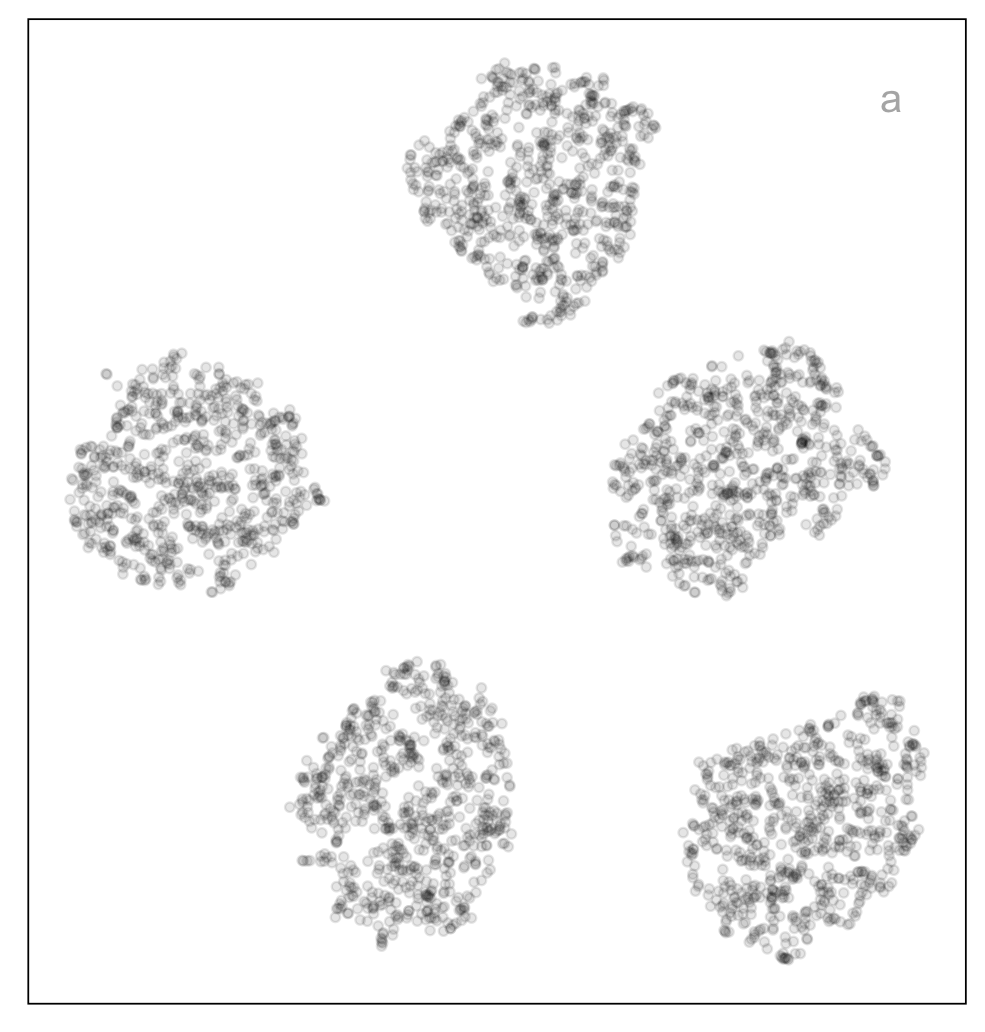
\includegraphics{figures/five_gau_clusters/tsne_layout.png}\end{minipage}%
%
\begin{minipage}{0.33\linewidth}
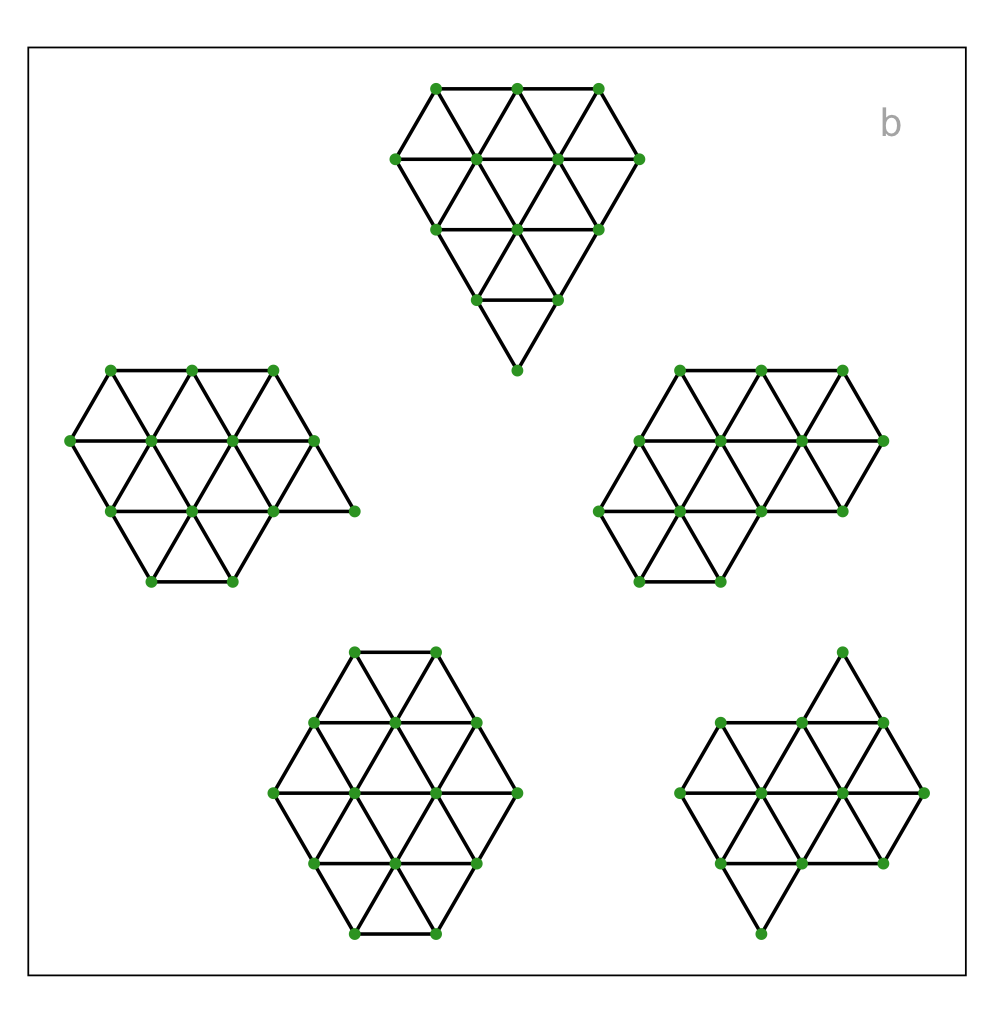
\includegraphics{figures/five_gau_clusters/2d_model_tsne.png}\end{minipage}%
%
\begin{minipage}{0.33\linewidth}
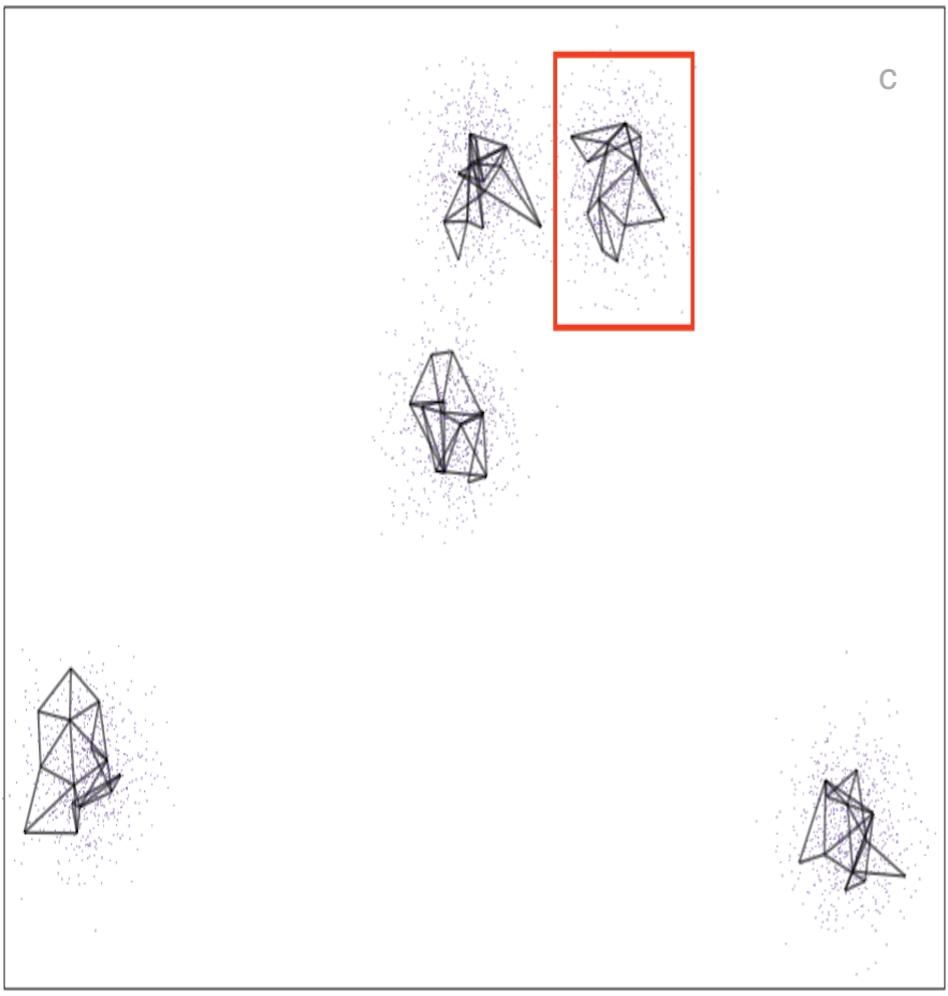
\includegraphics{figures/five_gau_clusters/sc_tsne_3.png}\end{minipage}%

\caption{\label{fig-gau-tsne-sc}The tSNE layout, model in \gD{}, and a
view of the fit in projections from \(4\text{-}D\), for the five
Gaussian cluster data. The model fits the separation and tries to
\emph{filled out} the clusters. (The \textbf{langevitour} software is
used to view the data with a tour, and the full video is available at
(\url{https://youtu.be/RASEE7N5MbM}).}

\end{figure}%

\begin{figure}[H]

\begin{minipage}{0.33\linewidth}
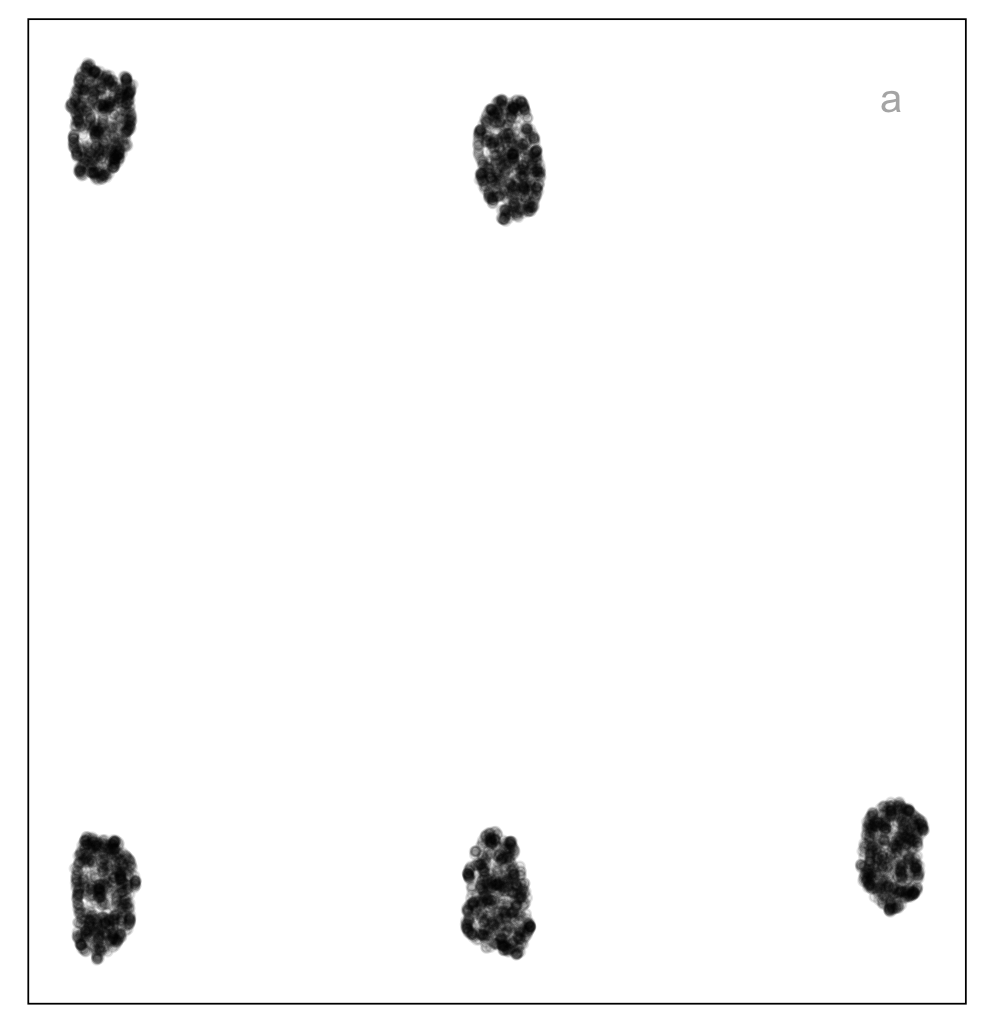
\includegraphics{figures/five_gau_clusters/umap_layout.png}\end{minipage}%
%
\begin{minipage}{0.33\linewidth}
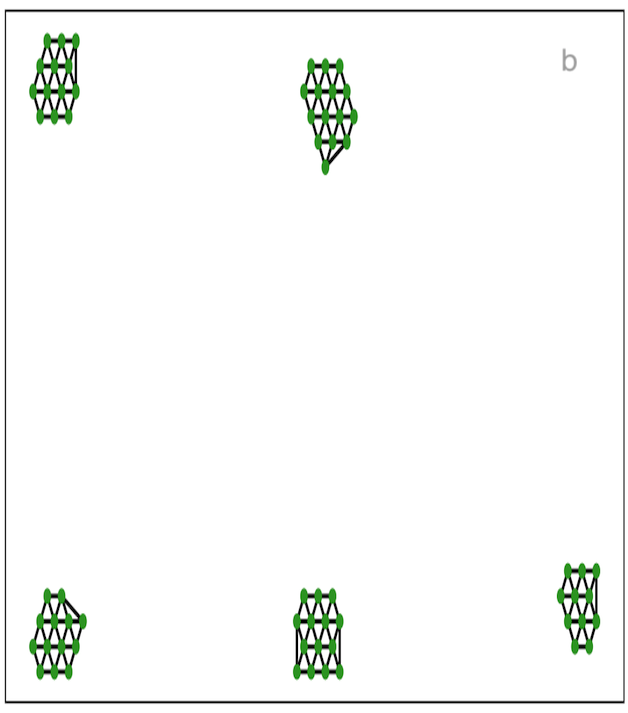
\includegraphics{figures/five_gau_clusters/2d_model_umap.png}\end{minipage}%
%
\begin{minipage}{0.33\linewidth}
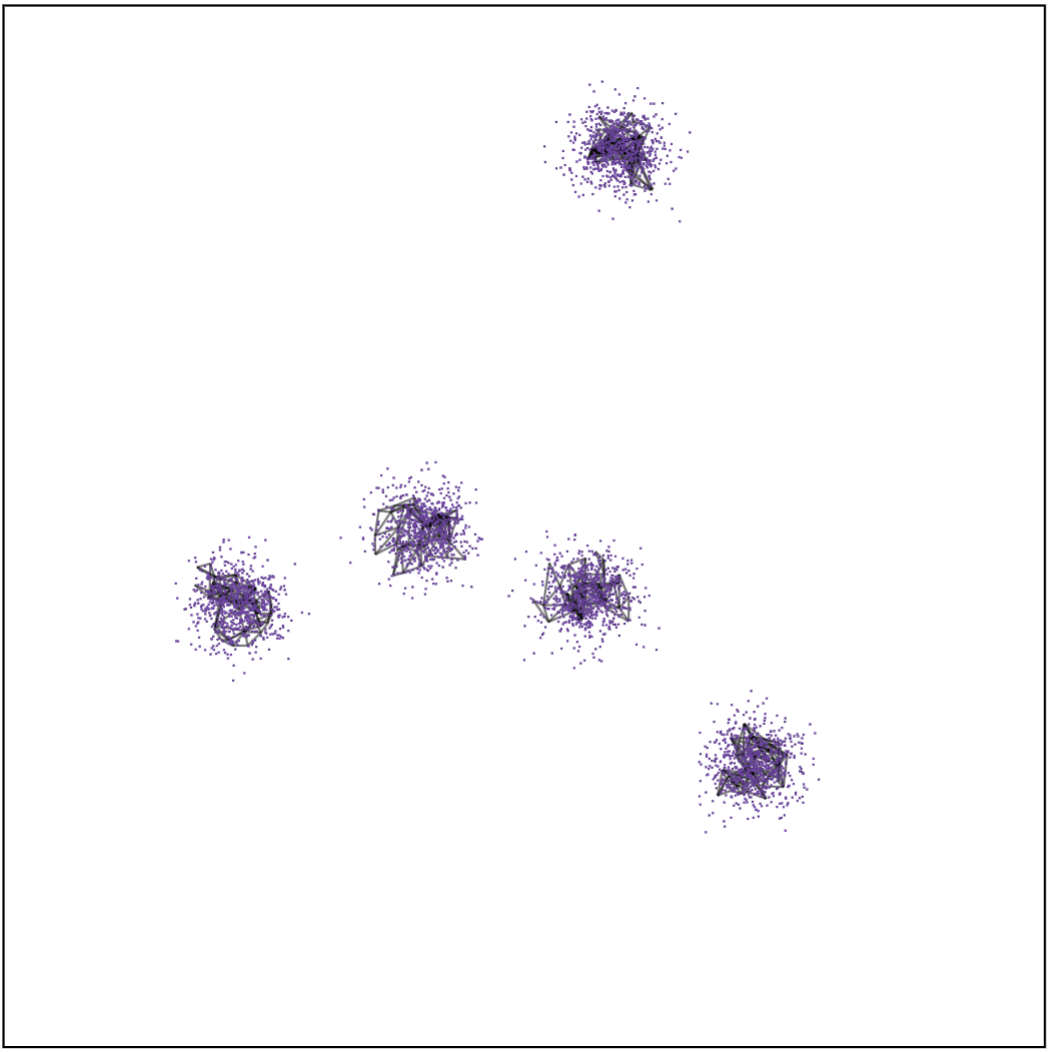
\includegraphics{figures/five_gau_clusters/sc_umap_3.png}\end{minipage}%

\caption{\label{fig-gau-umap-sc}The UMAP layout, model in \gD{}, and a
view of the fit in projections from \(4\text{-}D\), for the five
Gaussian cluster data. The model fits the separation and tries to
\emph{filled out} the clusters, but not as much as tSNE. (The
\textbf{langevitour} software is used to view the data with a tour, and
the full video is available at (\url{https://youtu.be/iG4bCPkJilw}).}

\end{figure}%

\begin{figure}[H]

\begin{minipage}{0.33\linewidth}
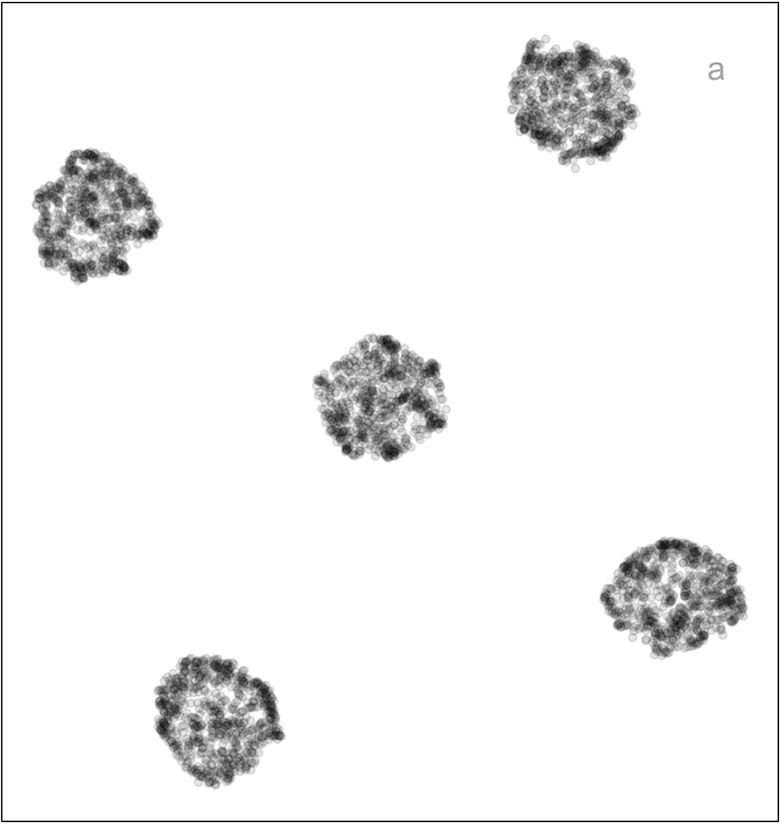
\includegraphics{figures/five_gau_clusters/pacmap_layout.png}\end{minipage}%
%
\begin{minipage}{0.33\linewidth}
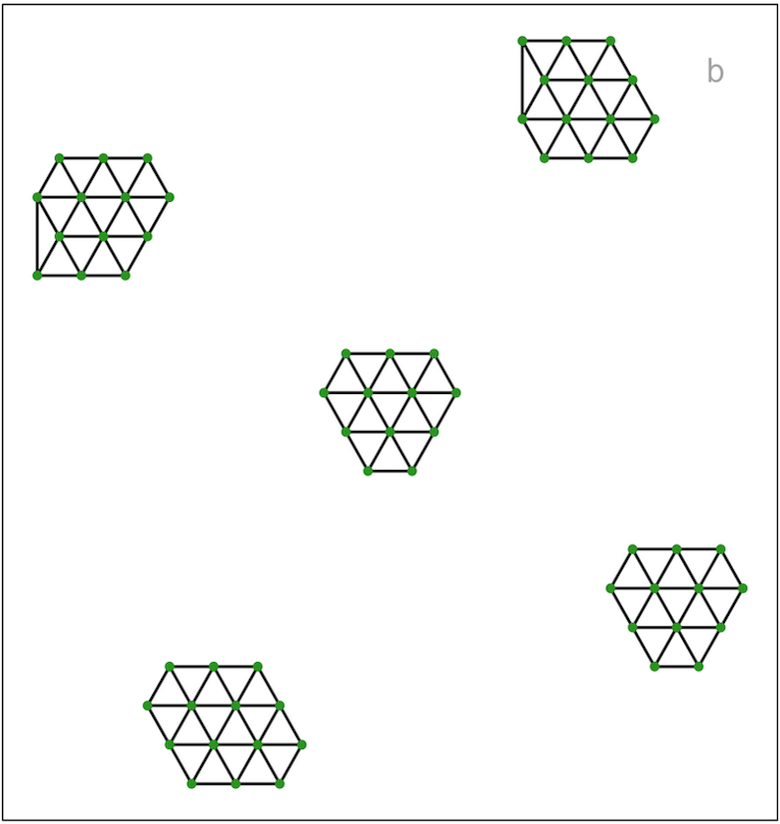
\includegraphics{figures/five_gau_clusters/2d_model_pacmap.png}\end{minipage}%
%
\begin{minipage}{0.33\linewidth}
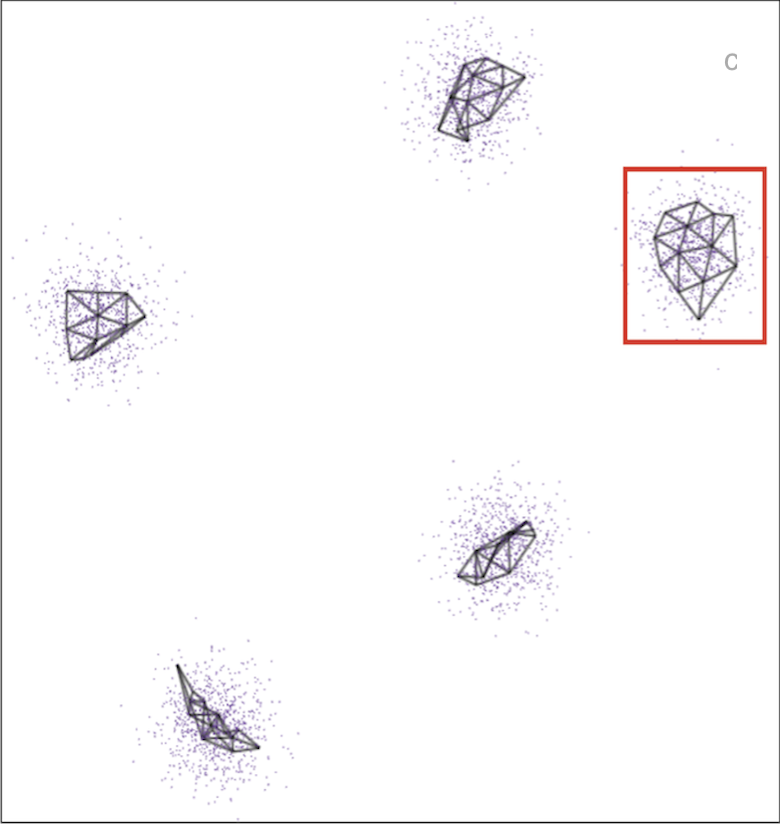
\includegraphics{figures/five_gau_clusters/sc_pacmap_2.png}\end{minipage}%

\caption{\label{fig-gau-pacmap-sc}The PaCMAP layout, model in \gD{}, and
a view of the fit in projections from \(4\text{-}D\), for the five
Gaussian cluster data. The model fits the separation and shows
\emph{flat} shaped clusters. (The \textbf{langevitour} software is used
to view the data with a tour, and the full video is available at
(\url{https://youtu.be/z07cKXi8EJQ}).}

\end{figure}%

\section{Applications}\label{sec-applications}

\subsection{Single-cell gene
expression}\label{single-cell-gene-expression}

In the field of single-cell studies, a common analytical task involves
clustering to identify groups of cells with similar expression profiles.
NLDR is commonly used to display clusters, and help to verify the
results. For example, \citet{chen2023} illustrates the use of UMAP to
identify clusters in Human Peripheral Blood Mononuclear Cells (PBMC3k).
Figure~\ref{fig-umap-author} is a reproduction of the published plot. It
shows three well-separated clusters.

\begin{figure}[H]

\centering{

\includegraphics[width=1\textwidth,height=0.3\textheight]{paper_files/figure-pdf/fig-umap-author-1.pdf}

}

\caption{\label{fig-umap-author}Reproduction of plot published in Chen
et al.~(2023) showing a \(2\text{-}D\) layout from UMAP applied for the
PBMC3k dataset. The (hyper-)parameter settings, beyond the defaults, are
30 nearest neighbors and minimum distance equal to 0.3. We use our
model-in-the-data-space to assess whether this is an accurate
representation of structure present in the high-dimensional data, or if
it is misleading.}

\end{figure}%

To determine whether the UMAP representation with the (hyper-)parameter
choice suggested by \citet{chen2023} preserves the original data
structure, we visualize the model constructed with UMAP overlaid on the
\pD{} data. The Figure~\ref{fig-umap-author} shows three well-separated
clusters. However, as shown in Figure~\ref{fig-pbmc1-sc}, there is no
big separation between three clusters in \pD{}. Therefore, the suggested
UMAP representation (Figure~\ref{fig-umap-author}) does not accurately
represent the structure(s) present in PBMC3k dataset. But, when
visualizing the model-in-th-data-space some unobserved structures can be
seen. Some clusters have non-linear continuity patterns and high-density
patches (Figure~\ref{fig-pbmc1-sc}).

XXXX I think we can remove the error figure, it's not part of the story

\begin{figure}[H]

\centering{

\includegraphics[width=1\textwidth,height=\textheight]{paper_files/figure-pdf/fig-model-pbmc-author-1.pdf}

}

\caption{\label{fig-model-pbmc-author}(a) Model generated in
\(2\text{-}D\) with UMAP, and (b) \(p\text{-}D\) model error in
\(2\text{-}D\). The \(2\text{-}D\) model shows three well-separated
distant clusters. The \(p\text{-}D\) model errors are distributed along
clusters.}

\end{figure}%

\begin{figure}[H]

\begin{minipage}{0.25\linewidth}
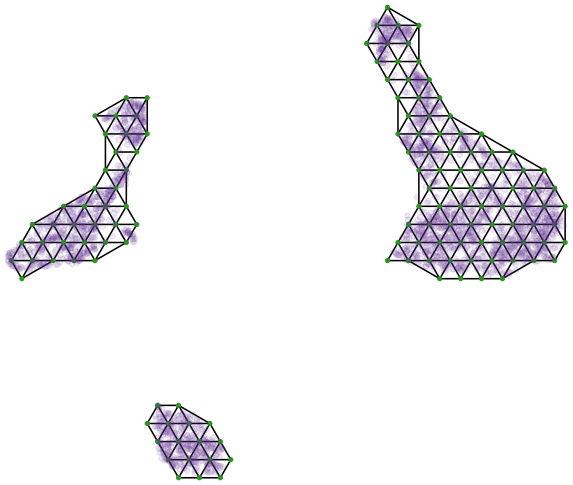
\includegraphics{figures/pbmc3k/umap_trimesh_plot.png}\end{minipage}%
%
\begin{minipage}{0.25\linewidth}
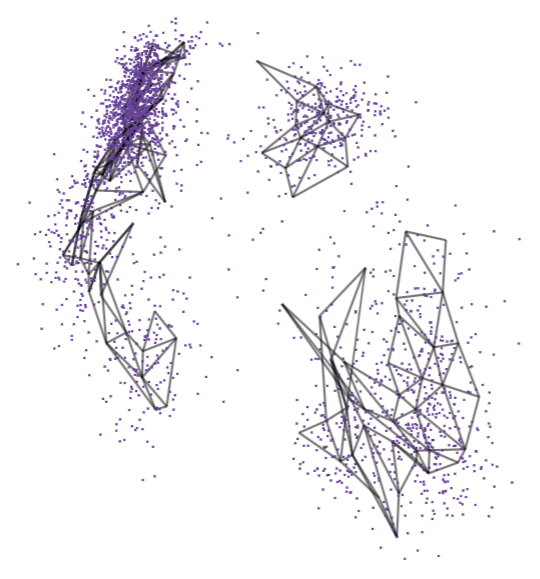
\includegraphics{figures/pbmc3k/sc_1.png}\end{minipage}%
%
\begin{minipage}{0.25\linewidth}
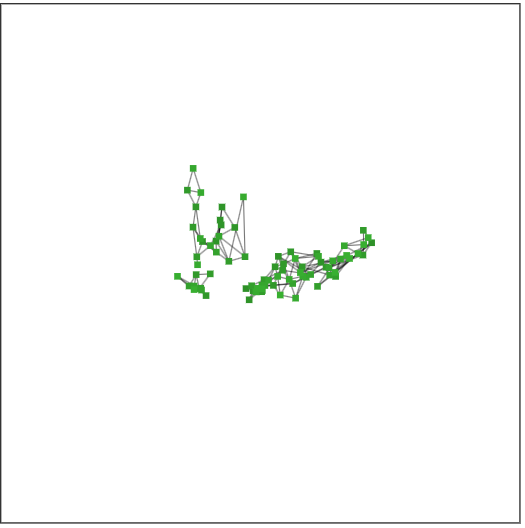
\includegraphics{figures/pbmc3k/sc_2.png}\end{minipage}%
%
\begin{minipage}{0.25\linewidth}
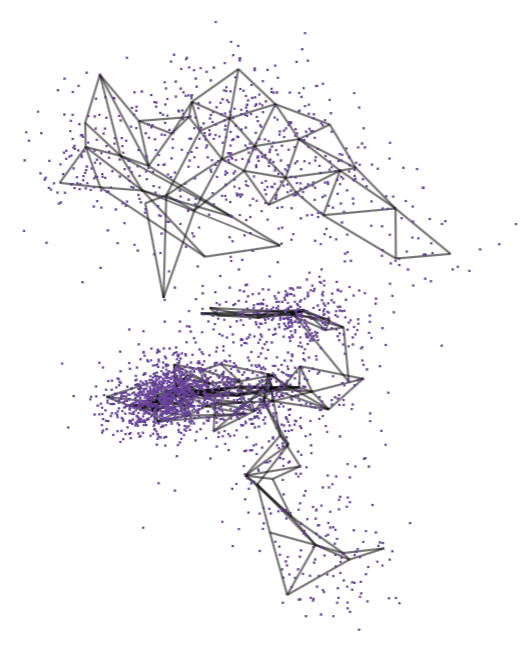
\includegraphics{figures/pbmc3k/sc_3.png}\end{minipage}%

\caption{\label{fig-pbmc1-sc}Model in \gD{}, on the UMAP layout, and
three views of the fit in projections from \(9\text{-}D\), for the
PBMC3k data (\((s_1, \ s_2) = (-0.050, \ -0.041)\),
\(b = 870 \  (30, \ 29)\), \(m = 135\), benchmark value to remove large
edges is \(0.099\)). (The \textbf{langevitour} software is used to view
the data with a tour, and the full video is available at
\url{https://youtu.be/VqqWuE0Jj6A}).}

\end{figure}%

In order to find a reasonable NLDR representation for the PBMC3k
dataset, the absolute error for different numbers of non-empty bins
using various NLDR techniques and different (hyper-)parameter settings
(Figure~\ref{fig-pbmc-abserror}) were calculated. After analyzing the
results, it was found that tSNE with default (hyper-)parameter setting
(perplexity: \(30\)) achieved the lowest error when there were \(136\)
number of non-empty bins. Therefore, tSNE with a perplexity value set to
\(30\), the default parameter setting, is considered as a reasonable
representation for the PBMC3k dataset.

\begin{figure}[H]

\centering{

\includegraphics[width=0.7\textwidth,height=\textheight]{paper_files/figure-pdf/fig-pbmc-abserror-1.pdf}

}

\caption{\label{fig-pbmc-abserror}Absolute error from UMAP and tSNE
applied to training PBMC3k dataset with diffferent parameter choices.
What is the best parameter choice to create the model? The residual plot
have a steep slope at the beginning, indicating that a smaller number of
non-empty bins causes a larger amount of error. Then, the slope
gradually declines or level off, indicating that a higher number of
non-empty bins generates a smaller error. Using the elbow method, it was
observed that when the number of non-empty bins is set to \(136\), the
lowest error occurred with the parameters perplexity: \(30\).}

\end{figure}%

As shown in Figure~\ref{fig-tsne-suggest}, there are three
well-separated clusters, although they are located close to each other.
Additionally, non-linear structures can also be observed within the
clusters (Figure~\ref{fig-tsne-suggest}). This demonstrates that tSNE
accurately captures the data structure of the PBMC3k dataset, which UMAP
did not achieve.

\begin{figure}[H]

\centering{

\includegraphics[width=0.4\textwidth,height=\textheight]{paper_files/figure-pdf/fig-tsne-suggest-1.pdf}

}

\caption{\label{fig-tsne-suggest}The \(2\text{-}D\) layout from tSNE
applied for the PBMC3k dataset. The default (hyper-)parameter setting is
a perplexity \(30\). We use our model-in-the-data-space to assess
whether this is an accurate representation of structure present in the
high-dimensional data, or if it is misleading.}

\end{figure}%

We then fit the model for tSNE, and visualize the resultant model in the
\pD{} data space. The model shows a quirk, as shown in
Figure~\ref{fig-pbmc2-sc}. All three clusters are connected by an edge
except the small and large clusters. Because the clusters are so close
in \gD{}, they attempt to maintain the structure in \pD{} as well. This
is evident that tSNE with perplexity \(30\) provides a reasonable
representation of PBMC3k data.

\begin{figure}[H]

\centering{

\includegraphics[width=1\textwidth,height=0.3\textheight]{paper_files/figure-pdf/fig-model-pbmc-1.pdf}

}

\caption{\label{fig-model-pbmc}(a) Model generated in \(2\text{-}D\)
with tSNE, and (b) \(p\text{-}D\) model error in \(2\text{-}D\). The
\(2\text{-}D\) model shows three well-separated distant clusters. The
\(p\text{-}D\) model errors are distributed along clusters, but most low
\(p\text{-}D\) model errors present in the large cluster.}

\end{figure}%

\begin{figure}[H]

\begin{minipage}{0.25\linewidth}
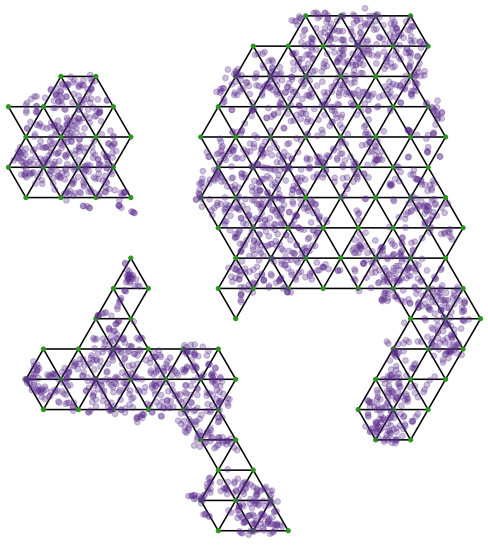
\includegraphics{figures/pbmc3k/tsne_trimesh_plot.png}\end{minipage}%
%
\begin{minipage}{0.25\linewidth}
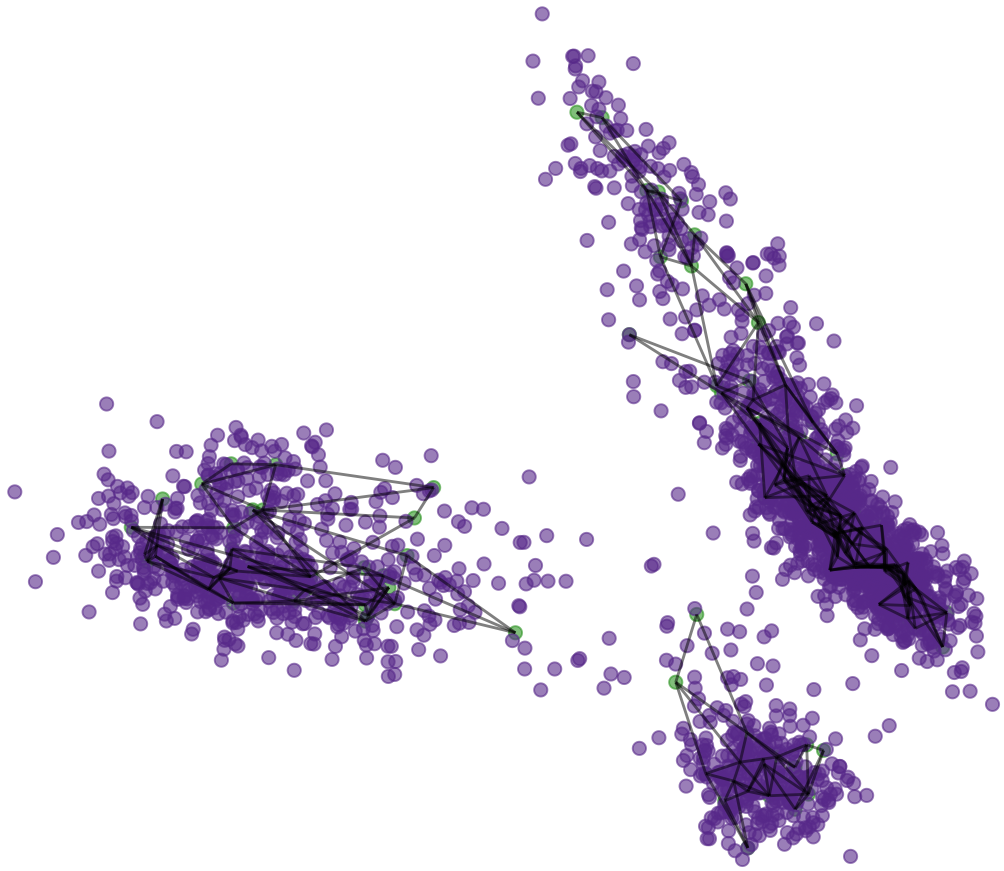
\includegraphics{figures/pbmc3k/sc_4.png}\end{minipage}%
%
\begin{minipage}{0.25\linewidth}
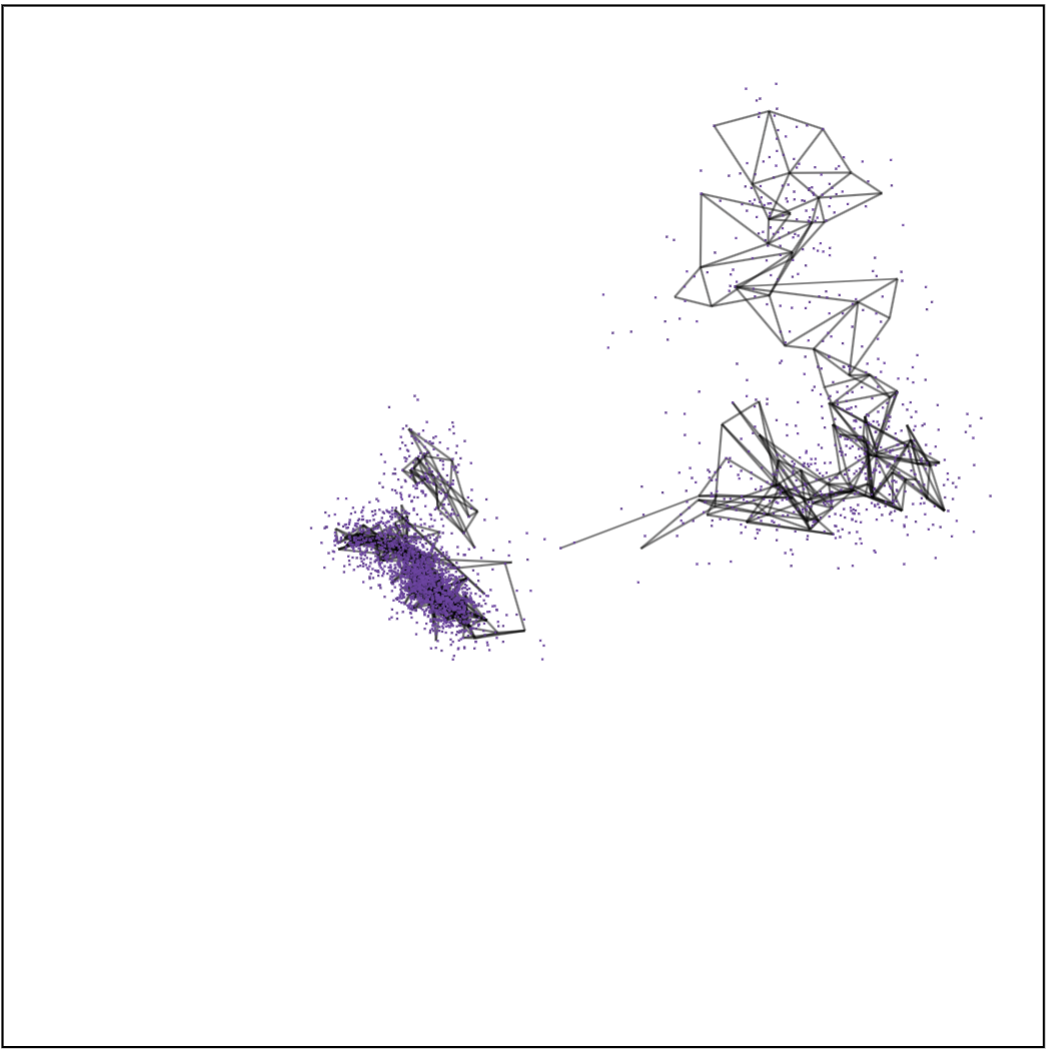
\includegraphics{figures/pbmc3k/sc_5.png}\end{minipage}%
%
\begin{minipage}{0.25\linewidth}
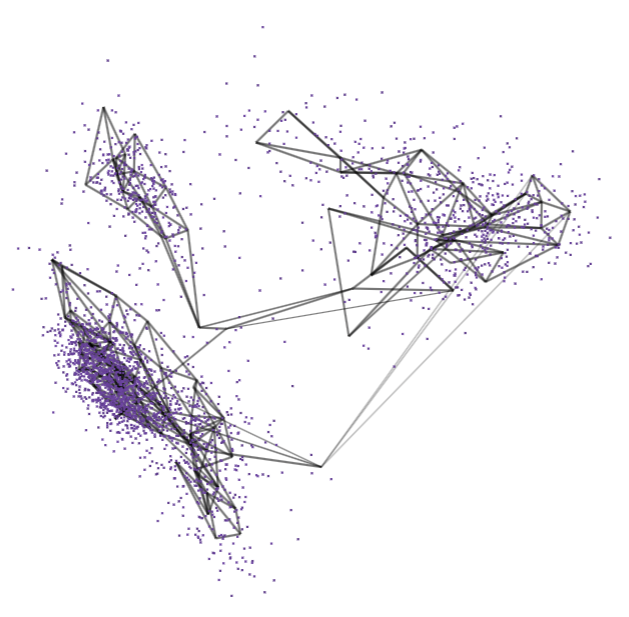
\includegraphics{figures/pbmc3k/sc_6.png}\end{minipage}%

\caption{\label{fig-pbmc2-sc}Model in \gD{}, on the tSNE layout, and
three views of the fit in projections from \(9\text{-}D\), for the
PBMC3k data (\((s_1, \ s_2) = (-0.050, \ -0.058)\),
\(b = 300 \  (15, \ 20)\), \(m = 136\), benchmark value to remove large
edges is \(0.133\)). (The \textbf{langevitour} software is used to view
the data with a tour, and the full video is available at
\url{https://youtu.be/5Y1hE4i7N2k}).}

\end{figure}%

\subsection{Hand-written digits}\label{hand-written-digits}

The MNIST dataset consists of grayscale images of handwritten digits
\citep{lecun2010}. \citet{yingfan2021} used this dataset to demonstrate
how PaCMAP preserves non-linear structure in \pD{}. To evaluate whether
PaCMAP provides a reasonable representation of the data, the \gD{}
embedding of the handwritten digit 1 was selected. As shown in
Figure~\ref{fig-pacmap-author}, the angle of the digit 1 images varies
along the \gD{} structure.

\begin{figure}[H]

\centering{

\includegraphics[width=1\textwidth,height=0.22\textheight]{paper_files/figure-pdf/fig-pacmap-author-1.pdf}

}

\caption{\label{fig-pacmap-author}\(2\text{-}D\) layout from PaCMAP
applied for the digit 1 of the MNIST dataset. The (hyper-)parameter
settings, beyond the defaults, are 10 nearest neighbors, ratio of the
number of mid-near pairs to the number of neighbors equal to 0.5, and
the ratio of the number of further pairs to the number of neighbors is
2. We use our model-in-the-data-space to assess whether this is an
accurate representation of structure present in the high-dimensional
data, or if it is misleading. The angle of the digit 1 varies along this
structure. Images at the top-left of the \(2\text{-}D\) layout show the
digit 1 angled more to the left, while images at the bottom-right show
the digit 1 angled more to the right.}

\end{figure}%

\begin{figure}[H]

\centering{

\includegraphics[width=1\textwidth,height=\textheight]{paper_files/figure-pdf/fig-model-mnist-1.pdf}

}

\caption{\label{fig-model-mnist}(a) Model generated in \(2\text{-}D\),
and (b) \(p\text{-}D\) model error in \(2\text{-}D\). The \(2\text{-}D\)
model shows a non-linear continuous structure. Most low \(p\text{-}D\)
model errors are distributed along the lower edge of the \(2\text{-}D\)
structure, while most high p-D model errors are concentrated along the
upper edge.}

\end{figure}%

According to Figure~\ref{fig-mnist1-sc1}, the non-linear continuous
structure observed in the \gD{} representation of PaCMAP
(Figure~\ref{fig-pacmap-author}) is also visible when visualizing the
model overlaid on the data space. This indicates that PaCMAP accurately
captures the structure of the \pD{} data. Additionally, the model shows
a twisted pattern within the non-linear structure in \pD{} space
(Figure~\ref{fig-mnist1-sc2}), which is an additional pattern not
visible in the \gD{} representation (Figure~\ref{fig-pacmap-author}).
Furthermore, as shown in Figure~\ref{fig-mnist1-sc3}, some long edges
exist in the \pD{} space that are not recognized as long edges in the
\gD{} representation. However, PaCMAP is a reasonable \gD{}
representation of MNIST digit 1 data, because PaCMAP preserves the
non-linear structure present in the \pD{} data.

\begin{figure}[H]

\begin{minipage}{0.25\linewidth}

\centering{

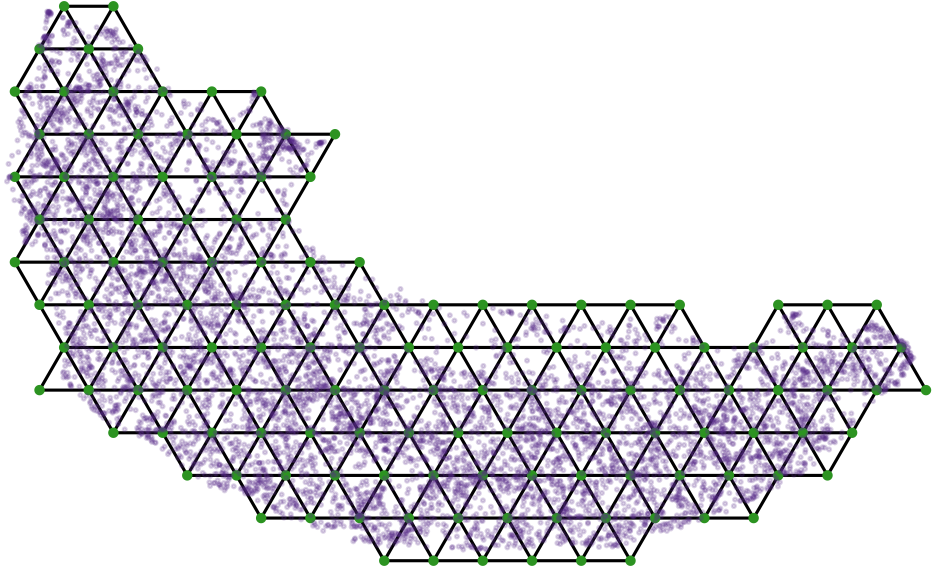
\includegraphics{figures/mnist/mnist_model_2d.png}

}

\subcaption{\label{fig-mnist1-model}}

\end{minipage}%
%
\begin{minipage}{0.25\linewidth}

\centering{

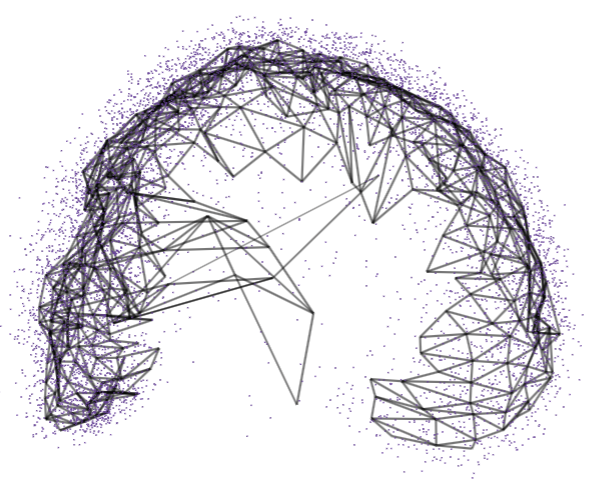
\includegraphics{figures/mnist/sc_1.png}

}

\subcaption{\label{fig-mnist1-sc1}}

\end{minipage}%
%
\begin{minipage}{0.25\linewidth}

\centering{

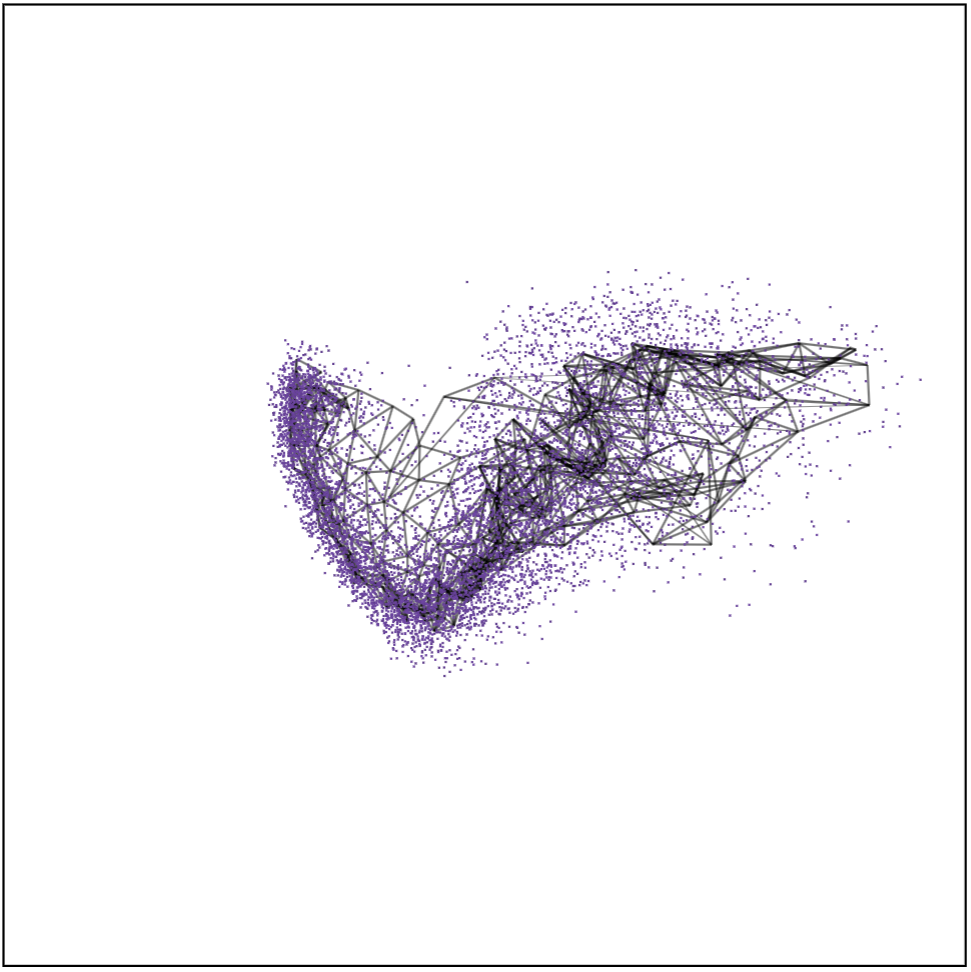
\includegraphics{figures/mnist/sc_2.png}

}

\subcaption{\label{fig-mnist1-sc2}}

\end{minipage}%
%
\begin{minipage}{0.25\linewidth}

\centering{

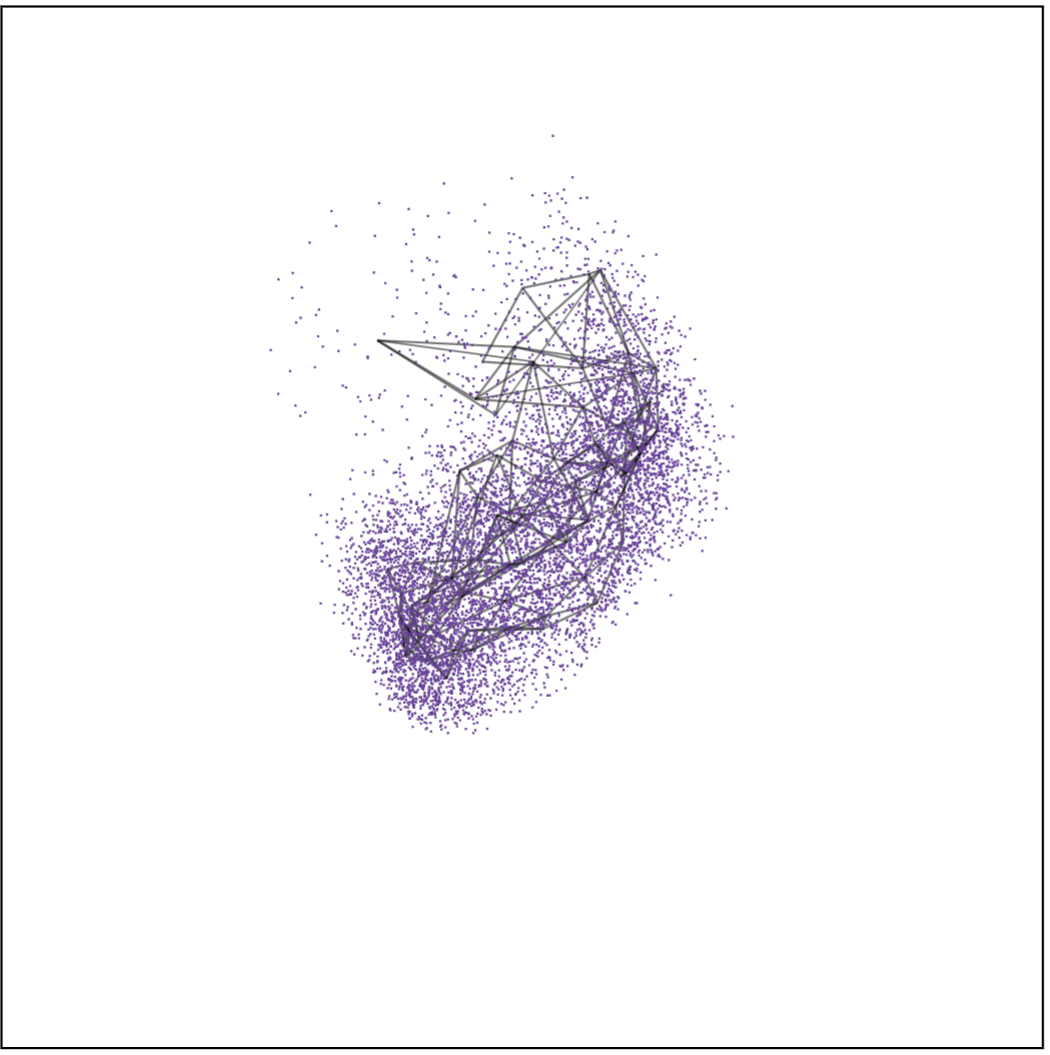
\includegraphics{figures/mnist/sc_3.png}

}

\subcaption{\label{fig-mnist1-sc3}}

\end{minipage}%

\caption{\label{fig-mnist1-sc}Model in \gD{}, on the PaCMAP layout, and
three views of the fit in projections from \(10\text{-}D\), for the
digit 1 of MNIST data (\((s_1, \ s_2) = (-0.100, \ -0.059)\),
\(b = 374 \  (22, \ 17)\), \(m = 140\), benchmark value to remove large
edges is \(0.094\)). (The \textbf{langevitour} software is used to view
the data with a tour, and the full video is available at
\url{https://youtu.be/zcg_GXBmqjA}).}

\end{figure}%

There are certain data points that exhibit high error rates due to their
deviation from the usual \pD{} data structure, which makes them
anomalies (Figure~\ref{fig-model-mnist} b). These anomalies can be
classified into two types: those that are anomalies within the
non-linear structure and those that lie outside of it. The images
associated with high model error points within the non-linear structure
display different patterns of the digit 1, as shown in
Figure~\ref{fig-mnist1-within}. However, when comparing these images to
the ones found outside of the non-linear structure, it becomes evident
that the latter display different patterns of the digit 1
(Figure~\ref{fig-mnist1-out}).

\begin{figure}[H]

\begin{minipage}{0.50\linewidth}

\centering{

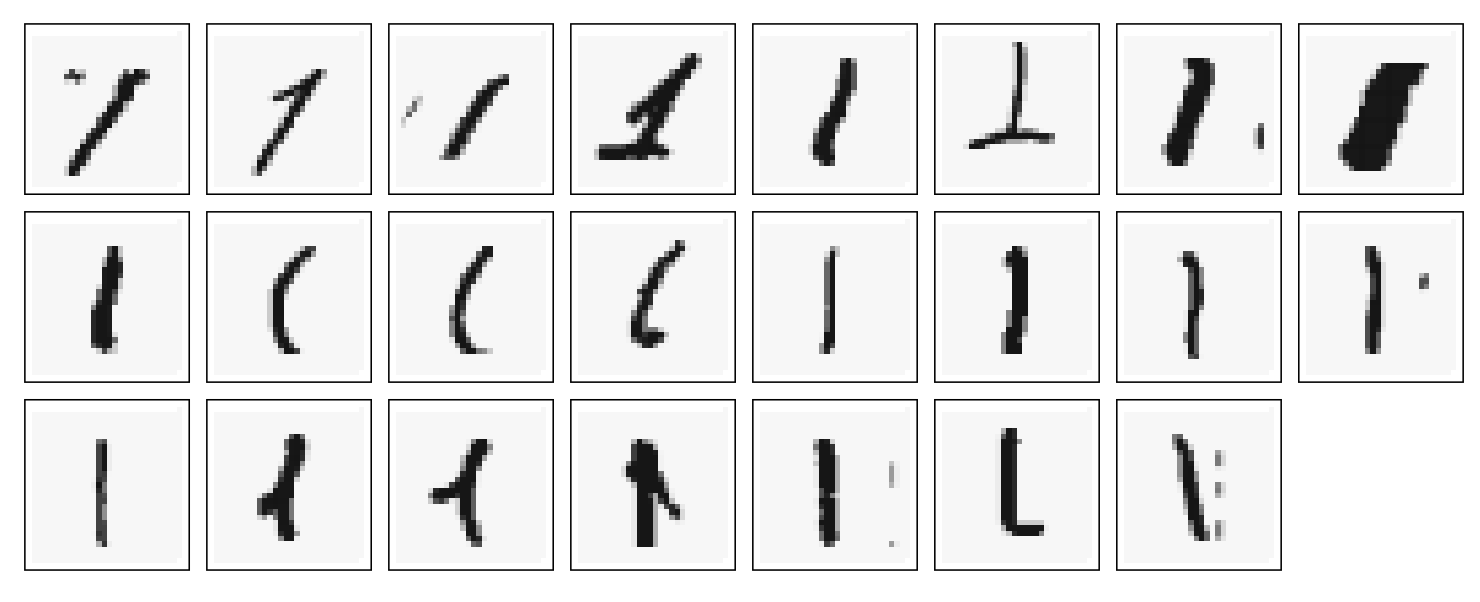
\includegraphics{figures/mnist/img_error_sample_within.png}

}

\subcaption{\label{fig-mnist1-within}}

\end{minipage}%
%
\begin{minipage}{0.50\linewidth}

\centering{

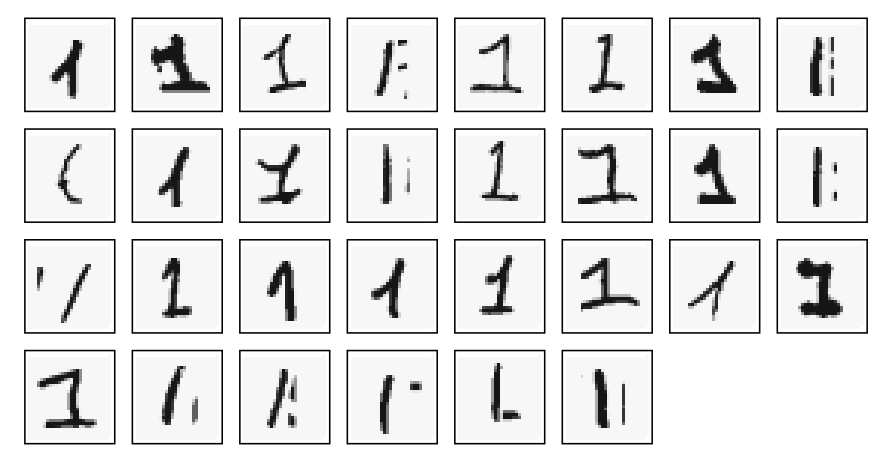
\includegraphics{figures/mnist/img_error_sample_out.png}

}

\subcaption{\label{fig-mnist1-out}}

\end{minipage}%

\caption{\label{fig-mnist-anomalies}Some images of handwritten digit 1
which occur high model error (a) within the non-linear structure, and
(b) outside the non-linear structure. The images shows different
patterns of digit 1.}

\end{figure}%

\section{Discussion}\label{sec-discussion}

This study makes several important contributions to the field of NLDR.
We have developed an algorithm to evaluate the most useful NLDR method
and (hyper-)parameter choices for creating a reasonable \gD{} layout of
high-dimensional data. Our objective is to fit a model for the \gD{}
layout that preserves the relationships between neighboring points and
turns it into a high-dimensional wireframe, which can be overlaid on the
data and visualized using a tour. This approach is defined as
\emph{model-in-data-space}. Viewing a model in the data space is an
ideal way to examine the fit.

The effectiveness of this approach is illustrated through various
examples. For instance, the S-curve example demonstrates how the model
accurately fits the points, capturing both local and global structures
in high-dimensional space. Our simulation case study further, five
Gaussian cluster example shows that while all observed NLDR methods
preserve the global structure, only tSNE effectively maintains the local
structure, highlighting the specific strengths and quirks of different
methods.

Human behavior often shows a desire for more certainty and a tendency to
prefer well-separated views. This emphasizes the importance of clear and
distinct clusters. For example, in the UMAP layout of the \textbf{pbmc}
dataset suggested by \citet{chen2023}, three distant, well-separated
clusters are shown. However, our model reveals that these clusters are
actually close to each other in \pD{}. Additionally, the model discovers
non-uniform data distribution and non-linear structures within the
clusters that are not visible in the UMAP layout, demonstrating the
ability of our model in uncovering hidden data characteristics.

Evaluating the error or unexplained variance is important for assessing
how well the model fits the data. By examining the error for different
numbers of bins, we found that tSNE with a perplexity of \(30\) provides
a reasonable representation for the \textbf{pbmc} dataset. Connecting
the closest clusters with line segments in the fitted model further
supports the preservation of neighborhood relationships.

The \textbf{digit: 1} example further illustrates the model's ability to
accurately capture non-linear structures and provide additional
information. Key findings include a twisted pattern that compresses the
structure in some projections and long line segments that detect
anomalies.

Predicting new observations in \kD{} is particularly valuable due to the
limitations of some NLDR methods, like tSNE, which don't provide a
straightforward method for prediction. As a result, our approach offers
a solution that capable of generating predicted \kD{} embedding
regardless of the NLDR method employed, effectively addressing this
functional gap.

In conclusion, while our method effectively captures and represents
high-dimensional data structures, further enhancements could involve
introducing approaches to bind the data, indicate line segments beyond
\gD{}, and diagnose the fitted model. These improvements would help in
creating a more accurate representation of the data when \gD{} layout is
inadequate.

\section{Supplementary Materials}\label{supplementary-materials}

Code, and data for reproducing this paper are available at
\url{https://github.com/JayaniLakshika/paper-nldr-vis-algorithm}.

\section*{References}\label{references}
\addcontentsline{toc}{section}{References}

\renewcommand{\bibsection}{}
\bibliography{bibliography.bib}

\newpage{}





\end{document}
